\chapter{Related Work} \label{chap:relatedwork}

\minitoc

Multi-granularity locking is a well-known solution to the problem of hierarchical locking in database systems. 
With MGL, locking a vertex in a hierarchy in a specific mode implicitly locks its descendants in the same mode. 
This is a powerful concept that allows for efficient locking of hierarchical data structures without the need to explicitly lock large portions of the hierarchy.
While powerful, implementing an MGL protocol that successfully achieves this goal is non-trivial. 
% The primary challenge is an efficient computation of the ancestor-descendant relationships in the hierarchy. 
% Along with this, there are other requirements that contribute to the performance trade-offs of the locking protocol. 


% Generally, any locking approach has certain requirements and balances trade-offs between performance and correctness.
% Hierarchical locking approaches utilize several clever tricks to identify lock granularities, place locks on the vertices of the hierarchy and to ensure that the locking protocol is safe, fair and does not lead to starvation. 

The different locking approaches discussed in this chapter use different mechanisms to address the requirements specified in Section \ref{chap:background}, each with its own trade-offs. 
It would be appropriate to claim that no approach is all encompassing and the choice of the locking approach depends on the specific requirements of the application and the hierarchy being used. We present the strengths, weaknesses and the niche occupied by each lock mechanism.

Finally, we present the trade-offs between them and motivate the need for a new hierarchical locking protocol which addresses the limitations of the existing protocols by classifying them into categories based on the requirements they fulfil.


\section{Classical locking approaches for connected data}

A common approach for synchronization in connected data, like lists and trees, is lock coupling \cite{DBLP:journals/acta/BayerS77}, also known as hand-over-hand locking. In hand-over-hand locking, a thread locks a vertex before traversing to one of its children in the structure, unlocking the parent once the child is locked. 
This allows for per vertex synchronization, which improves concurrency by permitting multiple threads to work on different parts of the hierarchy simultaneously. 
However, as \citet{LeisH019} show, lock coupling can lead to suboptimal locking performance on modern hardware.


An alternative to lock coupling, targeted specially for B-trees is a variant called B-Link tree \cite{LehmanY81}. A B-link tree is an extension of the B-tree data structure that adds sibling pointers to improve concurrency and simplify lock management in multithreaded environments. In a traditional B-tree, nodes are connected in a hierarchical structure with each node containing keys and pointers to child nodes, but concurrent modifications require complex locking strategies to maintain consistency. B-link trees address this by adding \emph{right-sibling} pointers between nodes at the same level, allowing threads to traverse the tree even during insertions or deletions without needing to lock the entire structure. This enables more efficient concurrent access, as threads encountering locked nodes can follow sibling links to find the next valid node. B-link trees require additional mechanisms to ensure that pointer updates are atomic since multiple threads may attempt to modify the same pointers concurrently. Additionally, this approach is only applicable to tree-based structures and is not be directly transferable to other hierarchical data models.


Classical locking techniques for hierarchical data structures are often designed with a synchronization hypothesis. A hypothesis defines how and when synchronization mechanisms (like locks, barriers, or other coordination tools) are applied to ensure threads or processes do not interfere with each other. Lock coupling uses a simple hypothesis that a thread must acquire a lock on a vertex before traversing to its children. B-link trees introduce a more sophisticated hypothesis by allowing threads to follow sibling pointers when encountering locked nodes, thus reducing contention and improving concurrency. Such design choices limit their use in general purpose applications where the topology of a linked structure is not known a priori. 

\section{Fixed-grain locking techniques}
Unlike classical approaches which define a specific synchronization mechanism, read/write locks are often appropriated for hierarchical data by associating a lock guard for a predefined set of lock targets. For example, a unique lock guard can be assigned for all vertices of the same depth from the root of the hierarchy. All vertices with the same depth, then belong to the same grain and this grain does not depend on the lock request.We refer to this as \emph{fixed-grain locking}. 
Fixed-grain locking has two extremes: We can either have a single lock guard for all the vertices in the hierarchy (coarse-grain locking) or a unique lock guard for each target vertex (fine-grain locking).


% \subsection{Level-based locks}
% Level-based locking is a synchronization technique employed in hierarchical data structures to control concurrent access by just utilizing their structure. Level-based locks form lock grains based on some topological property of the hierarchy.
% % Level-based locks are the simplest form of locking for uses where the hierarchy is known a priori and the semantic classification of the vertices is fixed. 
% % Fixed-grain locking associates a fixed guard with a set of target vertices in the hierarchy which from the grain of that guard.
% % The two extremes of locking discussed in Chapter \ref{chap:background} are variants of fixed-grain locking. 
% One approach to level-based locking is to associate a lock guard per level of the hierarchy. This level is determined by the depth of vertices in the hierarchy. All vertices with the same depth are associated with a single lock guard.
% As shown in Figure \ref{fig:level_locks}, the hierarchy is divided into levels based on the depth of the vertices and a lock guard is associated with each level. 
% This guard protects all vertices in that level.
% To lock a target vertex, a thread acquires the lock associated with the level of that target and locks all the vertices in that level.
% For example, in Figure \ref{fig:level_locks}, in order to lock target vertex $$\mathcal{D}$$, vertices $E$, $F$ and $G$ are implicitly locked as well since they are in the same level and protected by the same guard as $$\mathcal{D}$$.

% \begin{figure}[h]
%     \centering
%     \captionsetup{justification=centering}
%     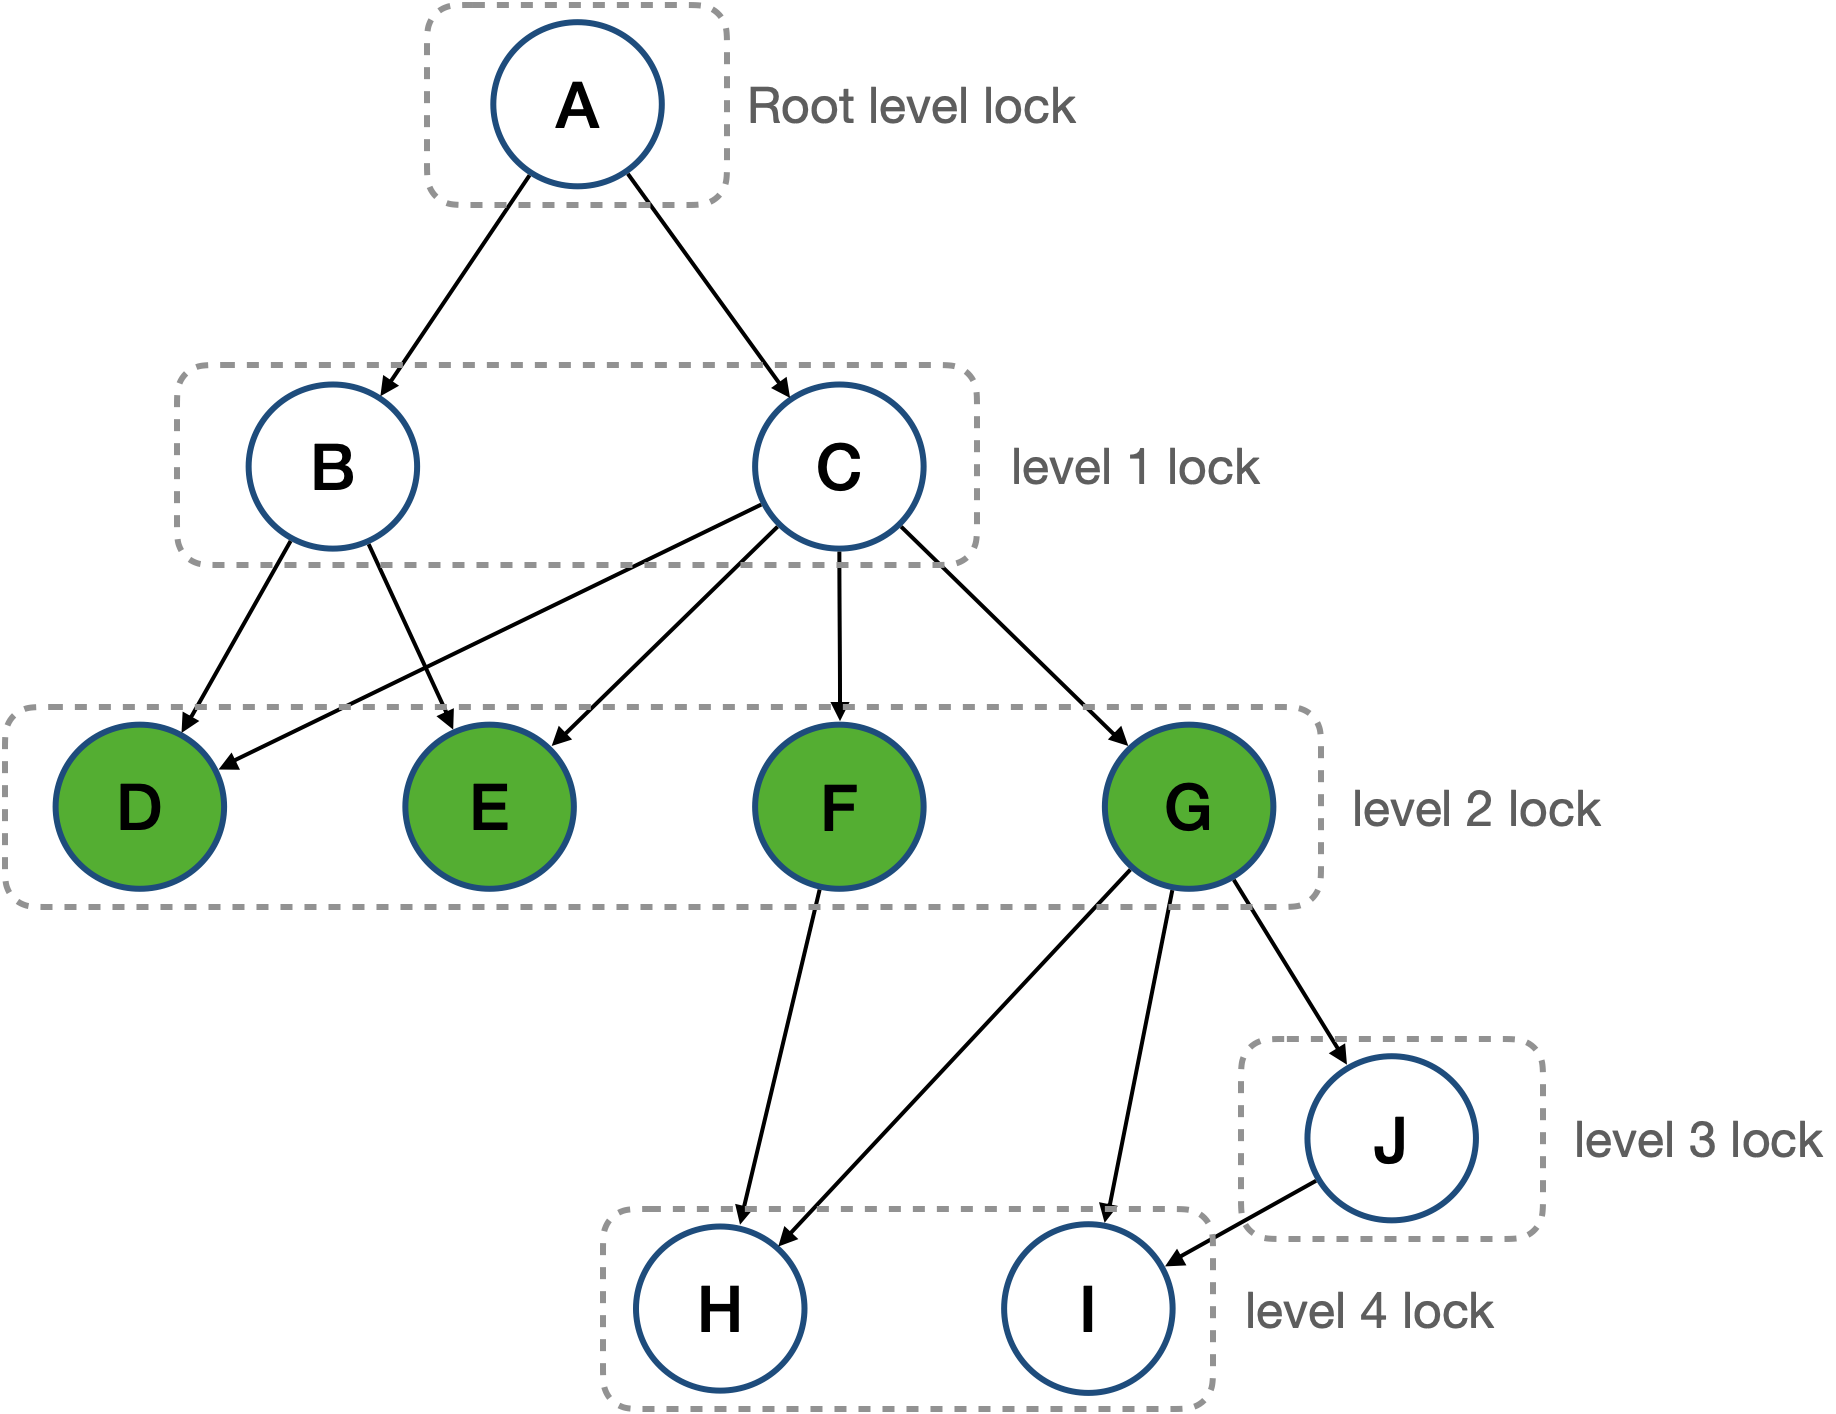
\includegraphics[width=0.7\textwidth]{figures/FixedGrainLevelLocks.png}
%     \caption{Hierarchical locks with fixed grains per level and a lock on level 2}
%     \label{fig:level_locks}
% \end{figure}

% Level-based locks fulfil only requirement \Rb since the lock guard is fixed for a set of vertices. 
% However, since the lock grain is fixed by level, acquiring a lock on a specific level implicitly locks all the vertices in that level. This leads to unnecessary conflicts between conflicts that access disjoint sets of vertices in the same level. 
% For example, consider two threads $T_1$ and $T_2$ that want to lock vertices $D$ and $E$ respectively.
% Since the lock guard for level 2 is the same, $T_1$ and $T_2$ will always conflict with each other even though they are accessing different vertices. 

% The lock guard for a request is not guaranteed to be optimal when using fixed-grain locks. 
% Depending on the lock grains chosen, the ancestor-descendant relationship may not be correctly identified. 
% This leads to unnecessary conflicts and can lead to performance degradation.
% For example, $D$ and $E$ are not related by an ancestor-descendant relationship and hence, under an effective MGL protocol, should not conflict.


% The granularity of a lock determines the degree of concurrency and the amount of contention in the system. 



\begin{figure}[H]
    \captionsetup{justification=centering}
    \centering
    \begin{subfigure}{.49\textwidth}
        \centering
        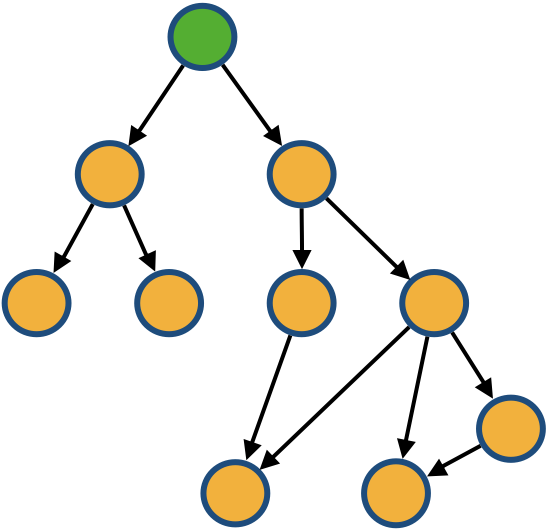
\includegraphics[width=.7\columnwidth]{figures/CoarseGrainedLockingTree}
        \caption{Coarse-grain lock}        
        \label{fig:fixedLockGrainsCoarse}
    \end{subfigure}
    \begin{subfigure}{.49\textwidth}
        \centering
        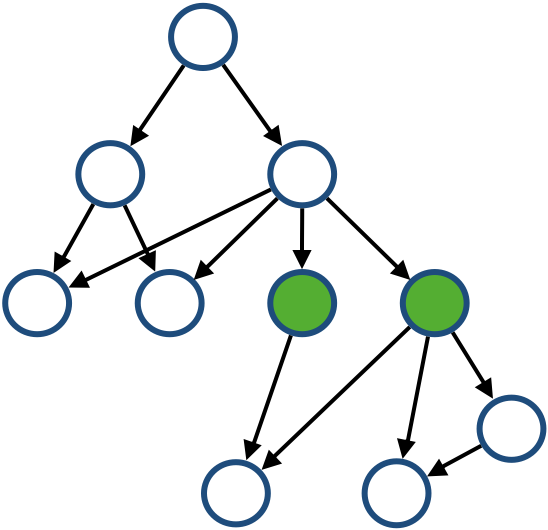
\includegraphics[width=.7\columnwidth]{figures/FineGrainLockingTree}
        \caption{Fine-grain locks}
        \label{fig:fixedLockGrainsFine}
    \end{subfigure}
    
    \label{fig:fixedLockGrains}
\caption{Fixed-grain locks in a hierarchical data structure (lock guard in green and the corresponding grain in yellow).}
\end{figure}


\subsection{Coarse-Grain Locking}
An oversimplified approach for correct thread synchronization is to guard an entire hierarchy with a single read-write lock such that any thread accessing the hierarchy must first acquire this lock.
This approach is called \emph{coarse-grain locking} and is shown in Figure \ref{fig:fixedLockGrainsCoarse}.
A thread that wishes to access any vertex in the hierarchy must first acquire a lock on the entire data structure and consequently block all other writers until it releases this lock. 
Coarse-grain locking is simple to implement and has extremely low locking overhead but suffers from the highest possible contention as all threads must acquire the same lock to access any part of the hierarchy. 


\subsection{Fine-Grain Locking}
Another well known approach to locking is to designate every target vertex as its own guard i.e. every vertex has its own unique lock. 
We call this \emph{fine-grain locking}.
As shown in Figure \ref{fig:fixedLockGrainsFine}, vertices are locked individually and a thread that needs to access multiple vertices must acquire multiple locks. 
Fine-grain locking has the advantage of reducing contention as threads can access disjoint parts of the hierarchy concurrently. 
However, the overhead of acquiring multiple locks makes this approach less efficient. 



% The approaches shown in Figures \ref{fig:fixedLockGrainsCoarse} and \ref{fig:fixedLockGrainsFine} have their own trade-offs. 
% Coarse-grain locking causes contention by unnecessarily blocking threads that access disjoint parts of the hierarchy. 
% Fine-grain locking, on the other hand, introduces significant overhead due to the need to acquire multiple locks for accessing multiple vertices with the additional requirement of deadlock detection and prevention/resolution.


% Another dimension of complexity with hierarchical data is the mutation of the hierarchy itself which causes topological changes.
% We refer to to such mutations as \emph{structural modifications}.
% Structural modifications, which alter the topology of a hierarchy are especially challenging for MGL techniques. 
% There already exist effective MGL protocols for hiaraarchies that do not undergo structural modifications, this is not the case for graphs whose structure can mutate. 
% We discuss this in Chapter \ref{chap:relatedwork}.
% A structural modification operation adds or removes vertices and{\slash}or edges and may conflict with ordinary operations, or with another structural modification.
% Such operations affect the identification of lock granules as their size and shape now depend on the new topology of the graph.



% \section{Related Work}
% Survey of existing research on locking mechanisms and optimization techniques. Comparison of related approaches to the CALock algorithm.



\section{Multi-granularity locking techniques}

In contrast to fixed-grain approaches, \emph{Multi-granularity locking} (MGL) \cite{gray1975granularity} adapts the granularity of locks based on the structure of the hierarchy and the lock request. 
According to \citet{gray1975granularity}, Multi-granularity locking involves locking a guard in a hierarchy such that a single lock guard is sufficient to protect all the target vertices protected by that guard i.e. a transaction that requests a write (exclusive) lock on a guard vertex implicitly exclusively locks all its targets when its request is granted. 

% A vertex which a thread intends to access is called the \emph{lock target} of the thread. 
% MGL methods generally associate a lock with each vertex in the hierarchy which we call the \emph{guard} of the vertex. 
% As such, when a thread wishes to access a target, it must acquire an appropriate lock on the guard of the the target vertex. 


 MGL techniques find a balance between the two extremes of fixed-grain locking based on the topology of the hierarchy.
% \emph{Multi-granularity locking} (MGL) \cite{gray1975granularity} techniques exploit the topology of the graph to identify a pertinent guard for a given target and aim to strike a balance between these two extremes. 
Since \emph{granularity} depends on the topology of the graph and on the lock request, lock requests with different lock targets can have different granularities, hence the name. A classical example of MGL is \emph{Intention locks} \cite{StonebrakerGranularity} which are often used in database indices to optimize hierarchical access \cite{sqlintentionlocks}. 

\begin{figure}[h]
    \captionsetup{justification=centering}
    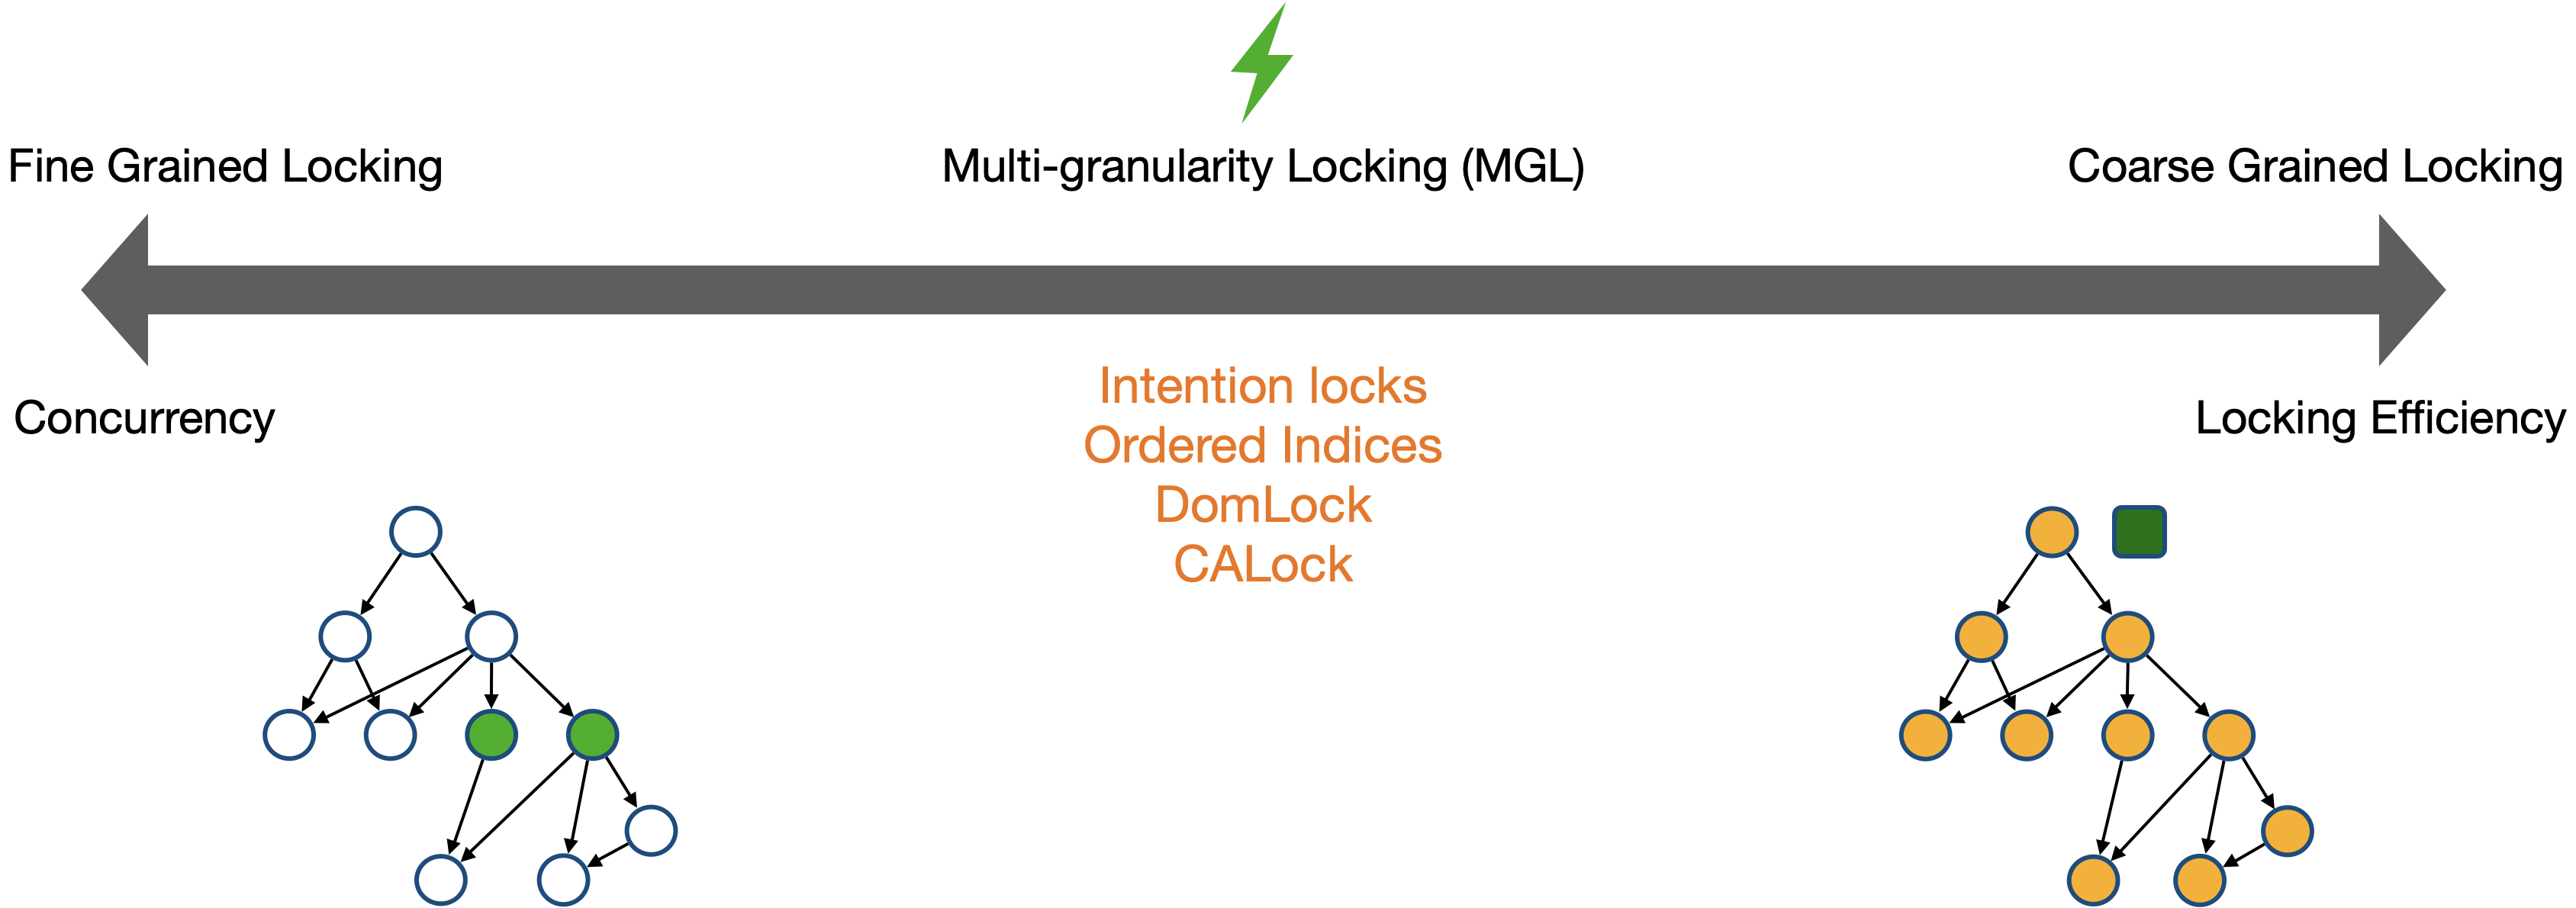
\includegraphics[width=\textwidth]{figures/MGLSpectrum.png}
    \label{fig:mglspectrum}
    \caption{Multi-Granularity locking provides a balance between Fine-grain and Coarse-grain locking.}
\end{figure}



\subsection{Intention Lock}

In order to lock a sub-graph rooted at a vertex $v$, it is necessary to prevent other threads from locking the ancestors of $v$ in shared or exclusive mode. To achieve this, \citet{gray1975granularity} introduced the concept of \emph{intention locks}. Intention locks are used to coordinate concurrent access by indicating a thread’s intention to acquire more fine-grain locks within a hierarchy. 


% Intention locks are used to coordinate concurrent access by indicating a thread’s intention to acquire more fine-grain locks within a hierarchy. Intention locks are acquired at higher levels of a hierarchy to signal that a thread is acquiring fine-grained locks on specific target vertices which exist deeper in the hierarchy. These intention locks protect the paths that lead to the target vertices from the root. By guarding these paths, intention locks ensure that the target vertices can be accesses exclusively by writers.

Intention locking was one of the first approaches to hierarchical locking designed to efficiently meet requirements \Rb and \Rc. Intention locking uses three new lock modes, IX (Intention Exclusive), IS (Intention Shared) and SIX (Shared with Intention Exclusive), which allow a thread to signify its intention to acquire an exclusive lock, a shared lock or a shared lock which can be upgraded to an exclusive lock on any descendant of the vertex locked under IX, IS or SIX modes, respectively. In the intention lock protocol, a thread acquires these intention locks on all vertices on all paths from the root to the lock target, which is then locked in either a shared (S) or exclusive (X) mode. Thus, all the ancestors of a target vertex are locked in an intention mode, and the target vertex is locked in a shared or exclusive mode.

The protocol requires that threads place these locks in a depth-first manner. This ordering ensures that two concurrent threads trying to lock the same target detect conflicts deterministically. Table \ref{tab:intention_locks} shows the compatibility matrix for the intention locks.


% Intention locking is one of the first approaches to hierarchical locking that attempts to address the requirements \Rb and \Rc with efficiency.
% \citet{gray1975granularity} introduce three new lock modes: IS (Intention Shared), IX (Intention Exclusive) and SIX (Shared Intention Exclusive) which signify the intention of a thread to acquire a shared or exclusive lock on a descendant of a vertex locked under IS, IX or SIX modes respectively.
% Intention lock protocol works by acquiring the aforementioned intention locks on the paths from the root to the lock target. The lock target is then locked in a shared (S) or exclusive (X) mode. These locks are always placed in a top-down, depth first manner. Owing to this, two concurrent threads, trying to lock the same lock target will always acquire the locks in the same order and detect a conflict. Table \ref{tab:intention_locks} shows the compatibility matrix for the intention locks.


\begin{table}[h]
    \centering
    \captionsetup{justification=centering}
    \begin{tabular}{c|ccccccc}
        \textbf{Mode} & \textbf{NL} & \textbf{IS} & \textbf{IX} & \textbf{S} & \textbf{SIX} & \textbf{X}\\
        \hline
        \textbf{NL} & \cellcolor{green!25} Y & \cellcolor{green!25} Y & \cellcolor{green!25} Y & \cellcolor{green!25} Y & \cellcolor{green!25} Y & \cellcolor{green!25} Y \\
        \textbf{IS} &  \cellcolor{green!25} Y & \cellcolor{green!25} Y & \cellcolor{green!25} Y & \cellcolor{green!25} Y & \cellcolor{green!25} Y & \cellcolor{red!25} N \\
        \textbf{IX} &  \cellcolor{green!25} Y & \cellcolor{green!25} Y & \cellcolor{green!25} Y & \cellcolor{red!25} N & \cellcolor{red!25} N & \cellcolor{red!25} N \\
        \textbf{S} &  \cellcolor{green!25} Y & \cellcolor{green!25} Y & \cellcolor{red!25} N & \cellcolor{green!25} Y & \cellcolor{red!25} N & \cellcolor{red!25} N \\
        \textbf{SIX} &  \cellcolor{green!25} Y & \cellcolor{green!25} Y & \cellcolor{red!25} N & \cellcolor{red!25} N & \cellcolor{red!25} N & \cellcolor{red!25} N \\
        \textbf{X} &  \cellcolor{green!25} Y & \cellcolor{red!25} N & \cellcolor{red!25} N & \cellcolor{red!25} N & \cellcolor{red!25} N & \cellcolor{red!25} N \\
    \end{tabular}
    \caption{Compatibility matrix for intention lock modes. \textbf{NL}: NoLock, \textbf{IS}: Intention Shared, \textbf{IX}: Intention Exclusive, \textbf{S}: Shared, \textbf{SIX}: Shared Intention Exclusive, \textbf{X}: Exclusive}
    \label{tab:intention_locks}
\end{table}



\begin{figure}[h]
    \centering
    \captionsetup{justification=centering}
    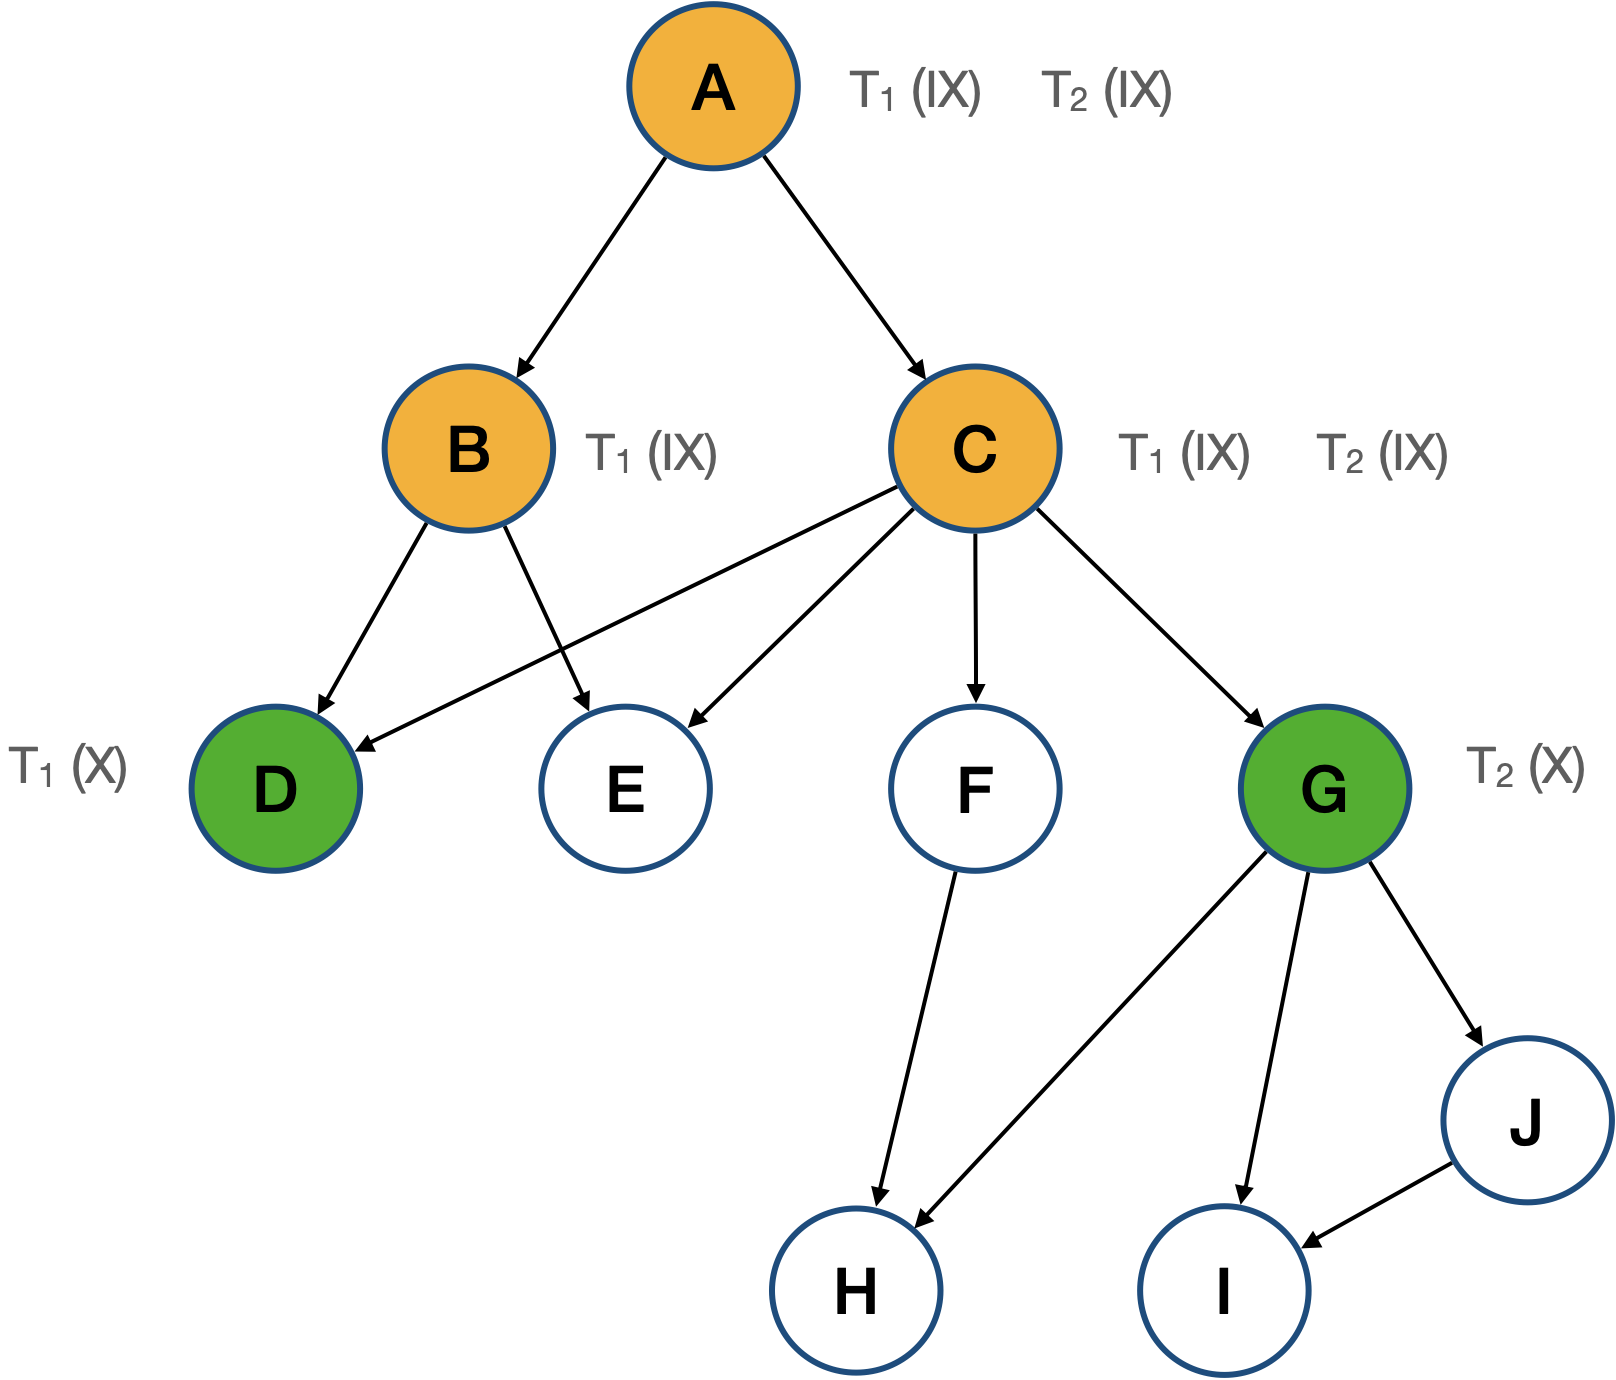
\includegraphics[width=0.6\textwidth]{figures/IntentionLockExample.png}
    \caption{Multi granularity locking via Intention locks. \\ $T_1$ takes an exclusive lock on vertex $D$ and $T_2$ takes an exclusive lock on vertex $G$ }
    \label{fig:intention_lock_example}
\end{figure}

Consider the example in Figure \ref{fig:intention_lock_example} where a thread $T_1$ wishes to acquire an exclusive lock (X) on target vertex $D$ and another thread, $T_2$ on target vertex $G$. 
% Since $D$ and $G$ are not related by an ancestor-descendant relationship, they should not conflict.
With intention locks, both threads start from the root ($A$) and acquire intention exclusive locks (IX) on the vertices from the root to their lock targets i.e. $D$ and $G$ respectively. 
Let's assume that $T_1$ is faster than $T_2$ and manages to acquire its locks first. 
$T_1$ acquires IX on vertices $A$, $B$ and $C$, in this order, and acquires an exclusive lock on $D$. 

When $T_2$ tries to acquire a lock on $G$, it acquires IX on vertices $A$ and $C$, in this order, before trying to acquire a lock on $G$. 
When $T_2$ tries to acquire a lock on $A$, it encounters a pre-existing  IX lock acquired by $T_1$. 
Since two IX locks are compatible, as seen in Table \ref{tab:intention_locks}, $T_2$ can acquire the IX lock on $A$.
Similarly, $T_2$ can acquire the IX lock on $C$ and then proceed to acquire an exclusive lock on $G$.


By locking the vertices on the path to the target vertex under IS and IX modes, always in a depth-first manner, 
intention locking protocol correctly identifies lock grain overlaps. 
However, this process requires multiple traversals from the root to the lock target so that all paths can be locked. 
In the example of Figure \ref{fig:intention_lock_example}, $T_1$ must perform the following two traversals:

\begin{itemize}
    \item $A \rightarrow B \rightarrow D$
    \item $A \rightarrow C \rightarrow D$
\end{itemize}

Once a thread has acquired the lock and performed the necessary accesses, it releases the locks from the leaves to the root. This again requires traversals. In the example in Figure \ref{fig:intention_lock_example}, $T_1$ must release the X locks on $D$ and $G$ respectively. Then backtrack towards the root to release the IX locks on $B$ and $C$ and finally release the IX lock on $A$. This involves the following two traversals:

\begin{itemize}
    \item $D \rightarrow B \rightarrow A$
    \item $D \rightarrow C \rightarrow A$
\end{itemize}




In a rooted tree, every vertex is reachable from the root via a unique path. 
This, however, is not the case with DAGs.
In DAGs, as the number of paths from the root to a target vertex increases, the number of traversals required to acquire and release an S or X lock on that vertex also increases because intention locks are to be acquired on all paths to the target vertex.
This leads to a significant performance degradation. Along with the added performance penalty, the order in which multiple paths are traversed needs to be deterministic to prevent deadlocks.  

So, while intention locks fulfil requirement \Rb, requirement \Rc incurs a significant performance penalty. 

\subsection{DomLock}
DomLock \cite{kalikar2016domlock} is a MGL technique that uses the concept of \emph{dominators} to identify lock grains instead of relying on explicitly locking paths that lead to a target. A dominator is a vertex that lies on all paths from the root to a target vertex $v$. A dominator is thus an effective lock guard for its descendants since, locking a dominator is sufficient to lock all the paths to $v$ (and the descendants of $v$).

\begin{definition}[Dominator]
    A vertex $d$ is a dominator of another vertex $v$ if all the paths from root to $v$ pass through d.
\end{definition}

A vertex can have several dominators. 
In order to maximize concurrency, DomLock uses the \emph{dominator of maximum depth} as the lock guard. This dominator is called the immediate dominator. 


% Dominator based locking (DomLock)  uses dominators to identify the ancestor descendant relationship in a hierarchy. DomLock finds a partial ordering of vertices in the hierarchy based on the ancestor-descendant relationship between them. To this end, DomLock uses the concept of dominators and immediate dominators. 


\begin{definition}[Immediate Dominator]
    Immediate Dominator: A dominator $\mathcal{D}$ is an immediate dominator of another vertex $v$ if there exists no other dominator for $v$ on the paths between $\mathcal{D}$ and $v$.
\end{definition}

This immediate dominator is the deepest vertex that lies on all paths from the root of the hierarchy to a target vertex. Therefore, it is sufficient to lock this immediate dominator to lock all the descendants since, any traversal to the target vertex or its descendants shall encounter the immediate dominator.

\subsubsection{Preprocessing and Metadata}

In order to identify the dominators of a vertex more efficiently, DomLock uses a labelling scheme that assigns a pair of integers to each vertex. This pair, called the \emph{interval} of a vertex $v$ is denoted  $I_v = [l_v, r_v]$. 
A vertex $u$ is a dominator of another vertex $v$ if the interval of $u$ ($I_u$) subsumes the interval of $v$ ($I_v$). Subsumption ($\prec$) is defined as follows.


% This interval $I_v$ subsumes  the intervals of all the descendants of $v$. Subsumption is defined as follows:
\begin{equation}
    u \text{ is a dominator of } v \iff I_u \prec I_v \iff l_v \leq l_u \land r_v \geq r_u
\end{equation}

% It is such that $l_v \leq l_u$ and $r_v \geq r_u$ for all vertices $u$ that are descendants of $v$. 

These intervals are computed by a post-order traversal of the hierarchy. Consider the example in Figure \ref{fig:domlock_example_locked}. A leaf is labelled with a unit interval. For example, vertex $D$ is labelled with the interval $[1, 1]$ since it is the first vertex in the post-order traversal.  

\begin{figure}
    \centering
    \captionsetup{justification=centering}
    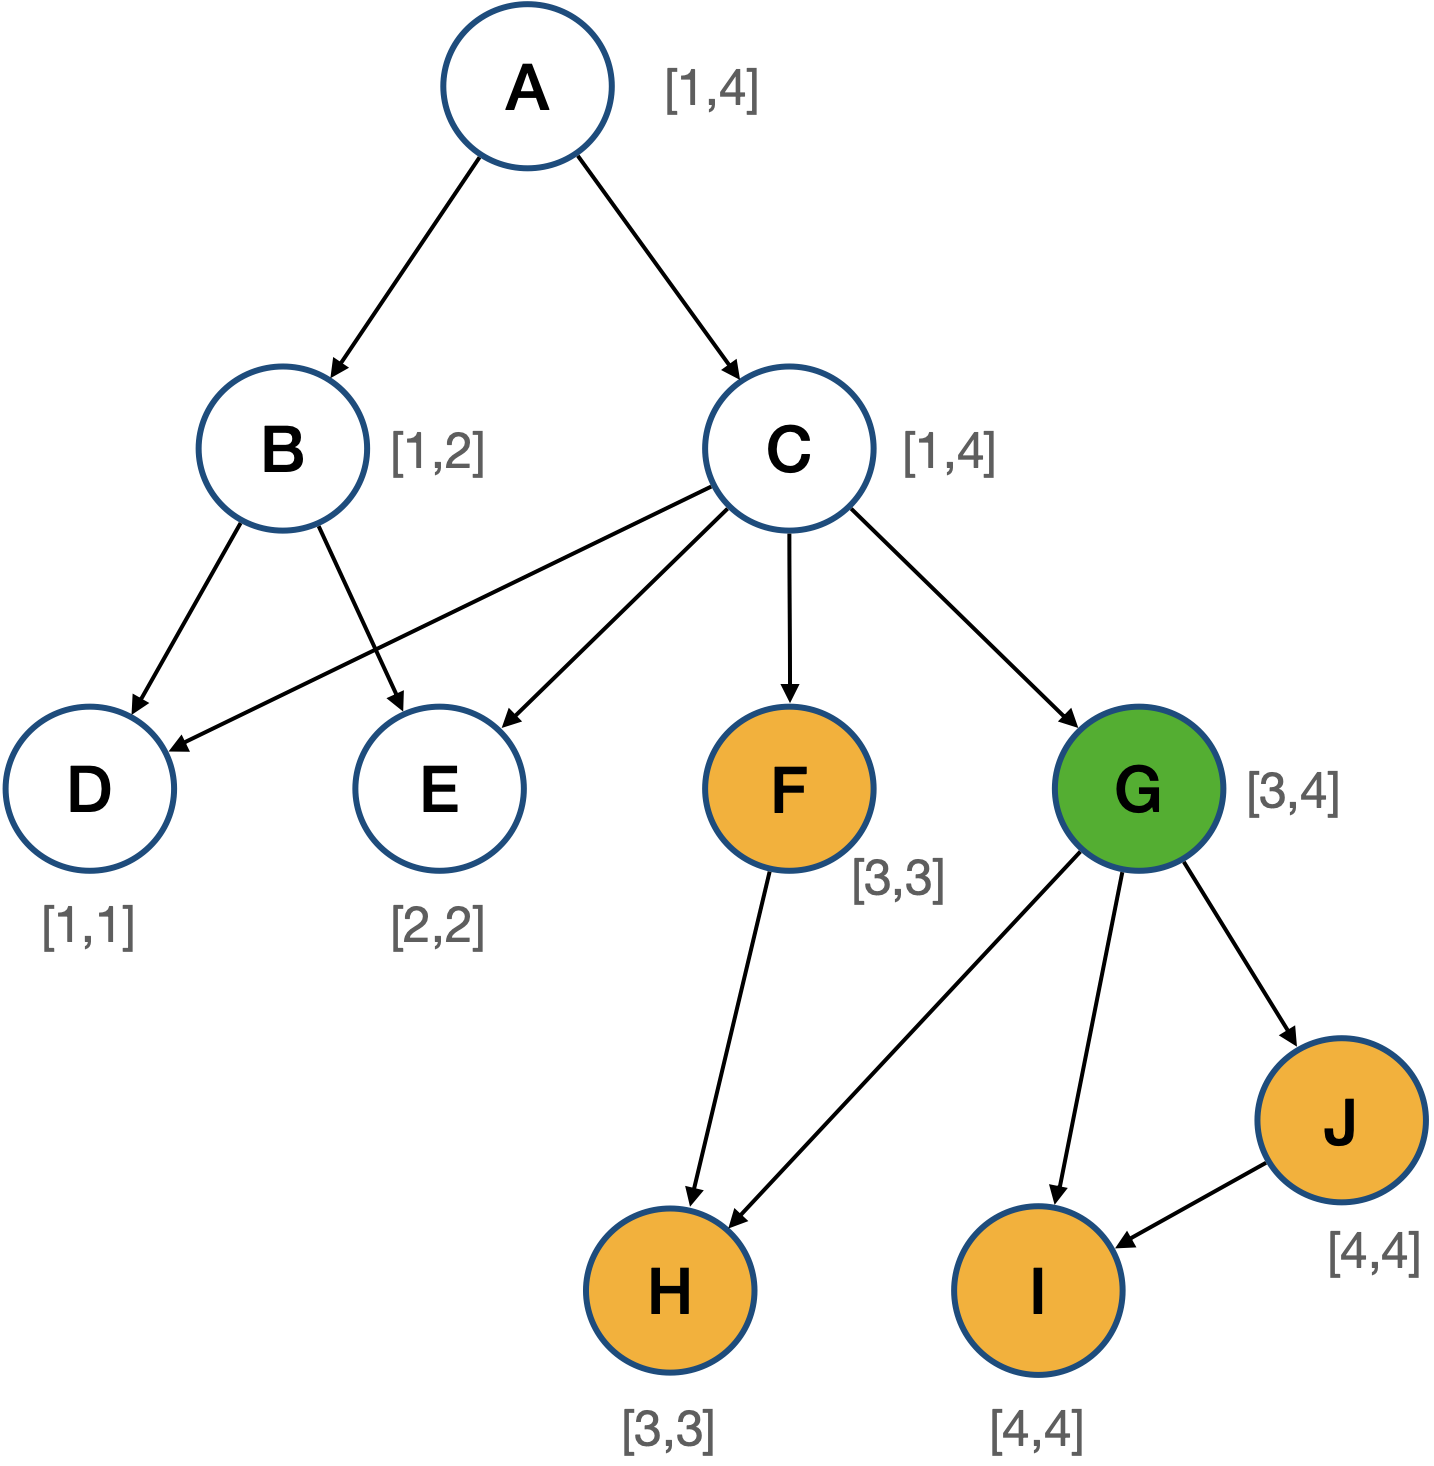
\includegraphics[width=.6\textwidth]{figures/domlock_example_with_lock.png}
    \caption{Hierarchy labelled with DomLock intervals and DomLock on $G$ (lock guard) with the grain of the grain of the lock (yellow).}
    \label{fig:domlock_example_locked}
\end{figure}

The interval of an internal vertex is computed from its children's. The $l$ value of an internal vertex $v$ is the minimum of the $l$ values of its children and its $r$ value is the maximum of the $r$ values of its children. For example, in Figure \ref{fig:domlock_example_locked}, vertex $G$ has three children $H$, $I$ and $J$. The interval of $G$ is $[3,4]$ since the minimum $l$ value of its children is 3 and the maximum $r$ value of its children is 4.  In turn, G is a dominator of \{H, I, J\}
% \begin{figure}[h]
%     \centering
%     \captionsetup{justification=centering}
%     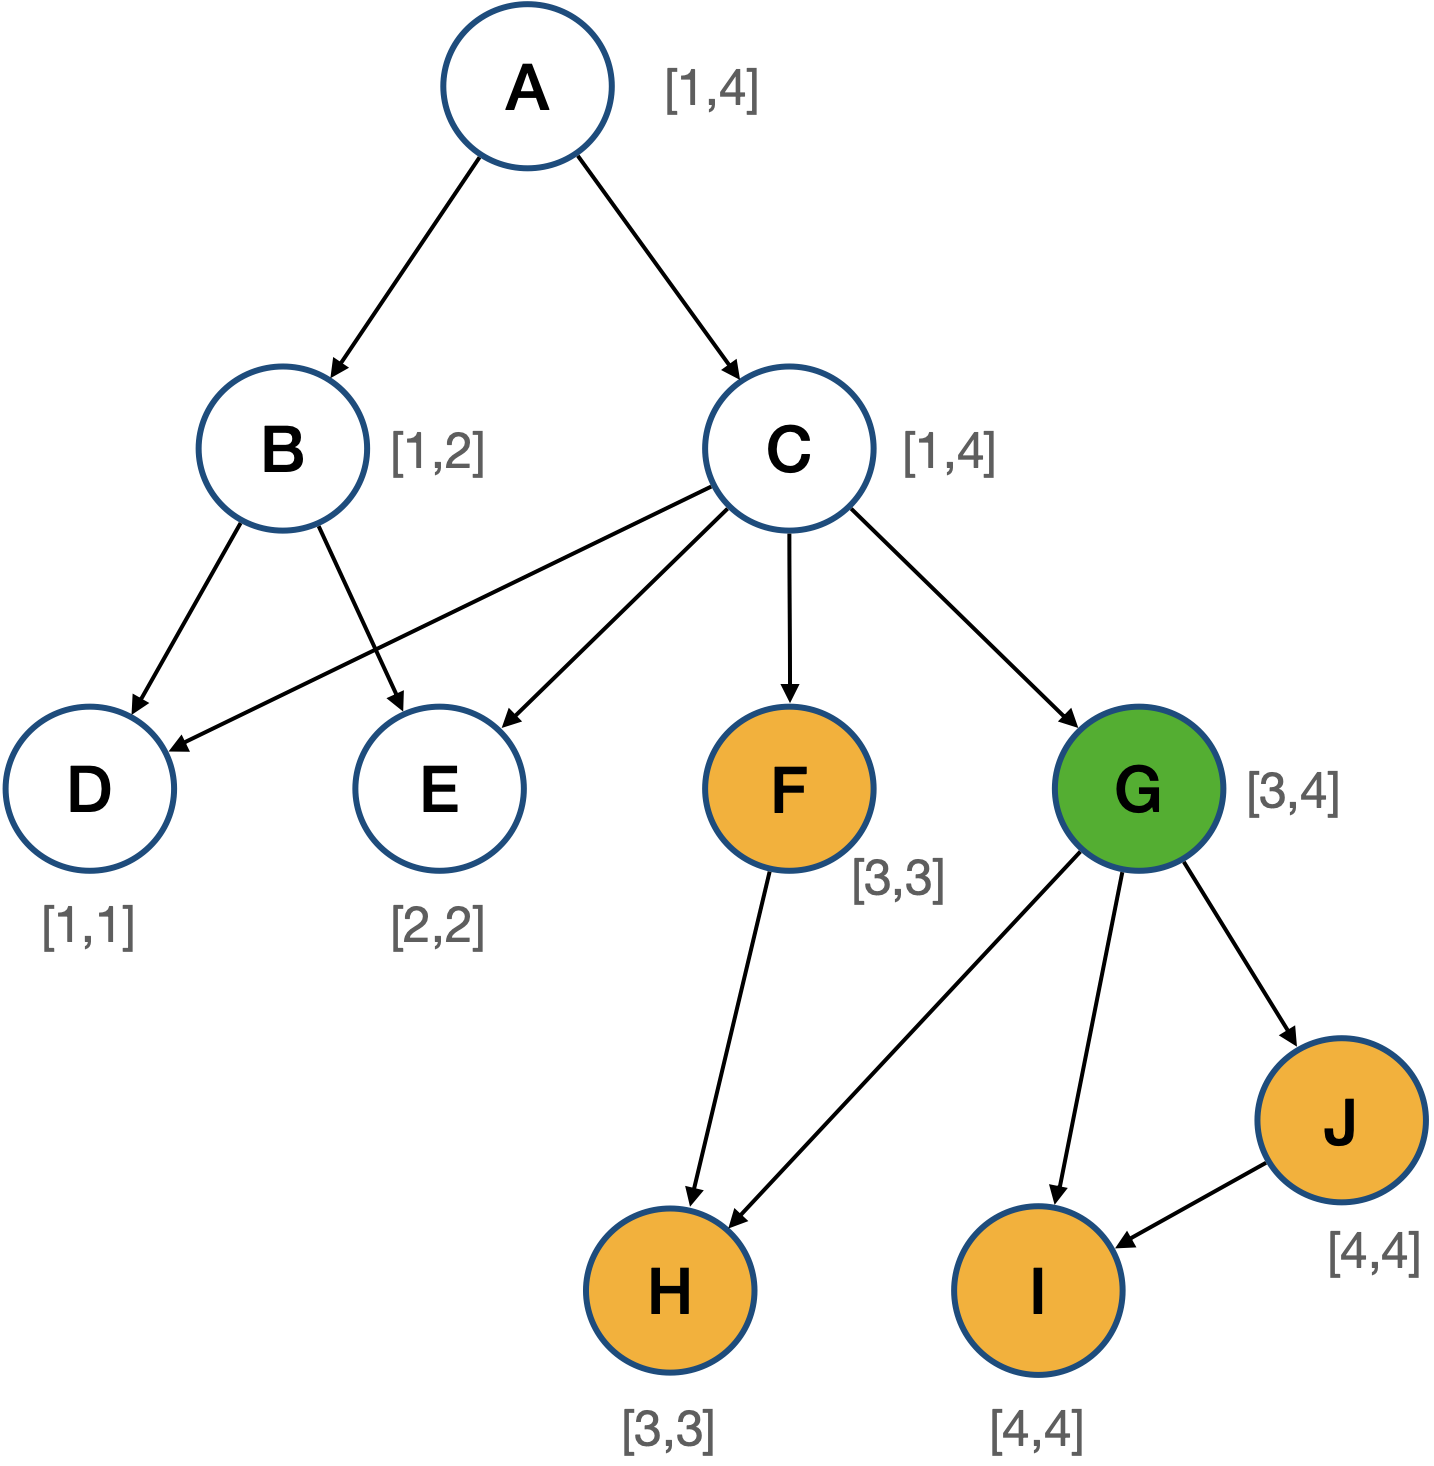
\includegraphics[width=0.5\textwidth]{figures/domlock_example_with_lock.png}
%     \caption{DomLock on guard $G$ with the grain of the grain of the lock (yellow).}
%     \label{fig:domlock_example_locked}
% \end{figure}

\subsubsection{Lock acquisition and Conflicts}

In order to identify the lock grain, DomLock uses the intervals of the targets of a lock request. Given a set of lock targets, the immediate dominator is chosen as the lock guards. This is done by finding the vertex with the smallest interval that subsumes the intervals of all lock targets.
Finding the immediate dominator involves a depth-first search from the root of the hierarchy.  

% Lock acquisition in DomLock uses the intervals of the vertices. The grain of a lock guard $g$ contains any vertex $v$ such that $v$ is a descendant of $g$ and $I_g \prec I_v$. 
% In practice, this involves a depth first search from the root of the hierarchy to identify the deepest vertex that satisfies the subsumption property to ensure that the granularity is as small as possible by locking the immediate dominator.
% A vertex $u$ subsumes another vertex $v$ when their intervals overlap i.e. $l_v \leq r_u \land l_u \leq r_v$. The lock grain of a guard $u$ is the set of vertices that have an overlapping interval with the interval of $u$. 


For example, in Figure \ref{fig:domlock_example_locked}, suppose a thread wants to acquire a lock on vertices $H$ and $J$ with intervals $[3,3]$ and $[4,4]$ respectively. The interval of the guard should subsume the intervals of $H$ and $J$. The smallest possible interval to achieve this is $[3,4]$. Now, a depth-first search is performed to identify the deepest vertex with interval $[3,4]$. DomLock identifies G as the lock guard for this lock request. The grain of $G$ contains $F$, $H$, $I$ and $J$ since the interval of $G$ subsumes the intervals of $F$, $H$, $I$ and $J$ which are $[3,3]$, $[3,3]$, $[4,4]$ and $[4,4]$ respectively.

By using numeric intervals, DomLock approximates the ancestor-descendant relationship in the hierarchy. The subsumption property aims to ensure that the interval of a vertex $v$ only subsumes the intervals of all its descendants. However, this is not always the case. 
Intervals are assigned by a post-order traversal. These intervals, in certain cases, provide false positives when identifying the ancestor-descendant relationship. We call such false positives, \emph{False subsumptions}. 
% Subsumption is a property that exists between two vertices related via an ancestor-descendant relationship. 
A false subsumption occurs when the intervals of two vertices overlap, but they are not related by an ancestor-descendant relationship. 
For example, in Figure \ref{fig:domlock_example_locked}, $G$ is a dominator of $F$ but $F$ is not a descendant of $G$. 
Sometimes, due to a false subsumption disjoint subgraphs are locked together since they are associated with the same lock guard. 
This leads to spurious lock conflicts and consequently, performance degradation. 

In order to test for a \textbf{grain conflict} between two lock requests, the intervals of the lock guards of the two requests are compared. Overlapping intervals indicate a conflict. For example, in Figure \ref{fig:domlock_example_locked}, along with a lock on G, another lock can be acquired on B since the intervals $[3,4]$ and $[1,2]$ respectively, do not overlap. However, a lock on C will conflict with a lock on G since the interval of C ($[1,4]$) overlaps with the interval of G ($[3,4]$).

\subsubsection{Metadata Maintainance}

Another drawback of DomLock is that it does not support dynamic hierarchies without having to relabel a large part of the hierarchy.
Since intervals are used to identify lock grains, they have to be recomputed when a structural modification occurs.
% The intervals of the vertices are computed once via a post-order traversal. When a vertex is added or removed from the hierarchy, this computation has to be redone. 

\begin{figure}[h]
    \centering
    \captionsetup{justification=centering}
    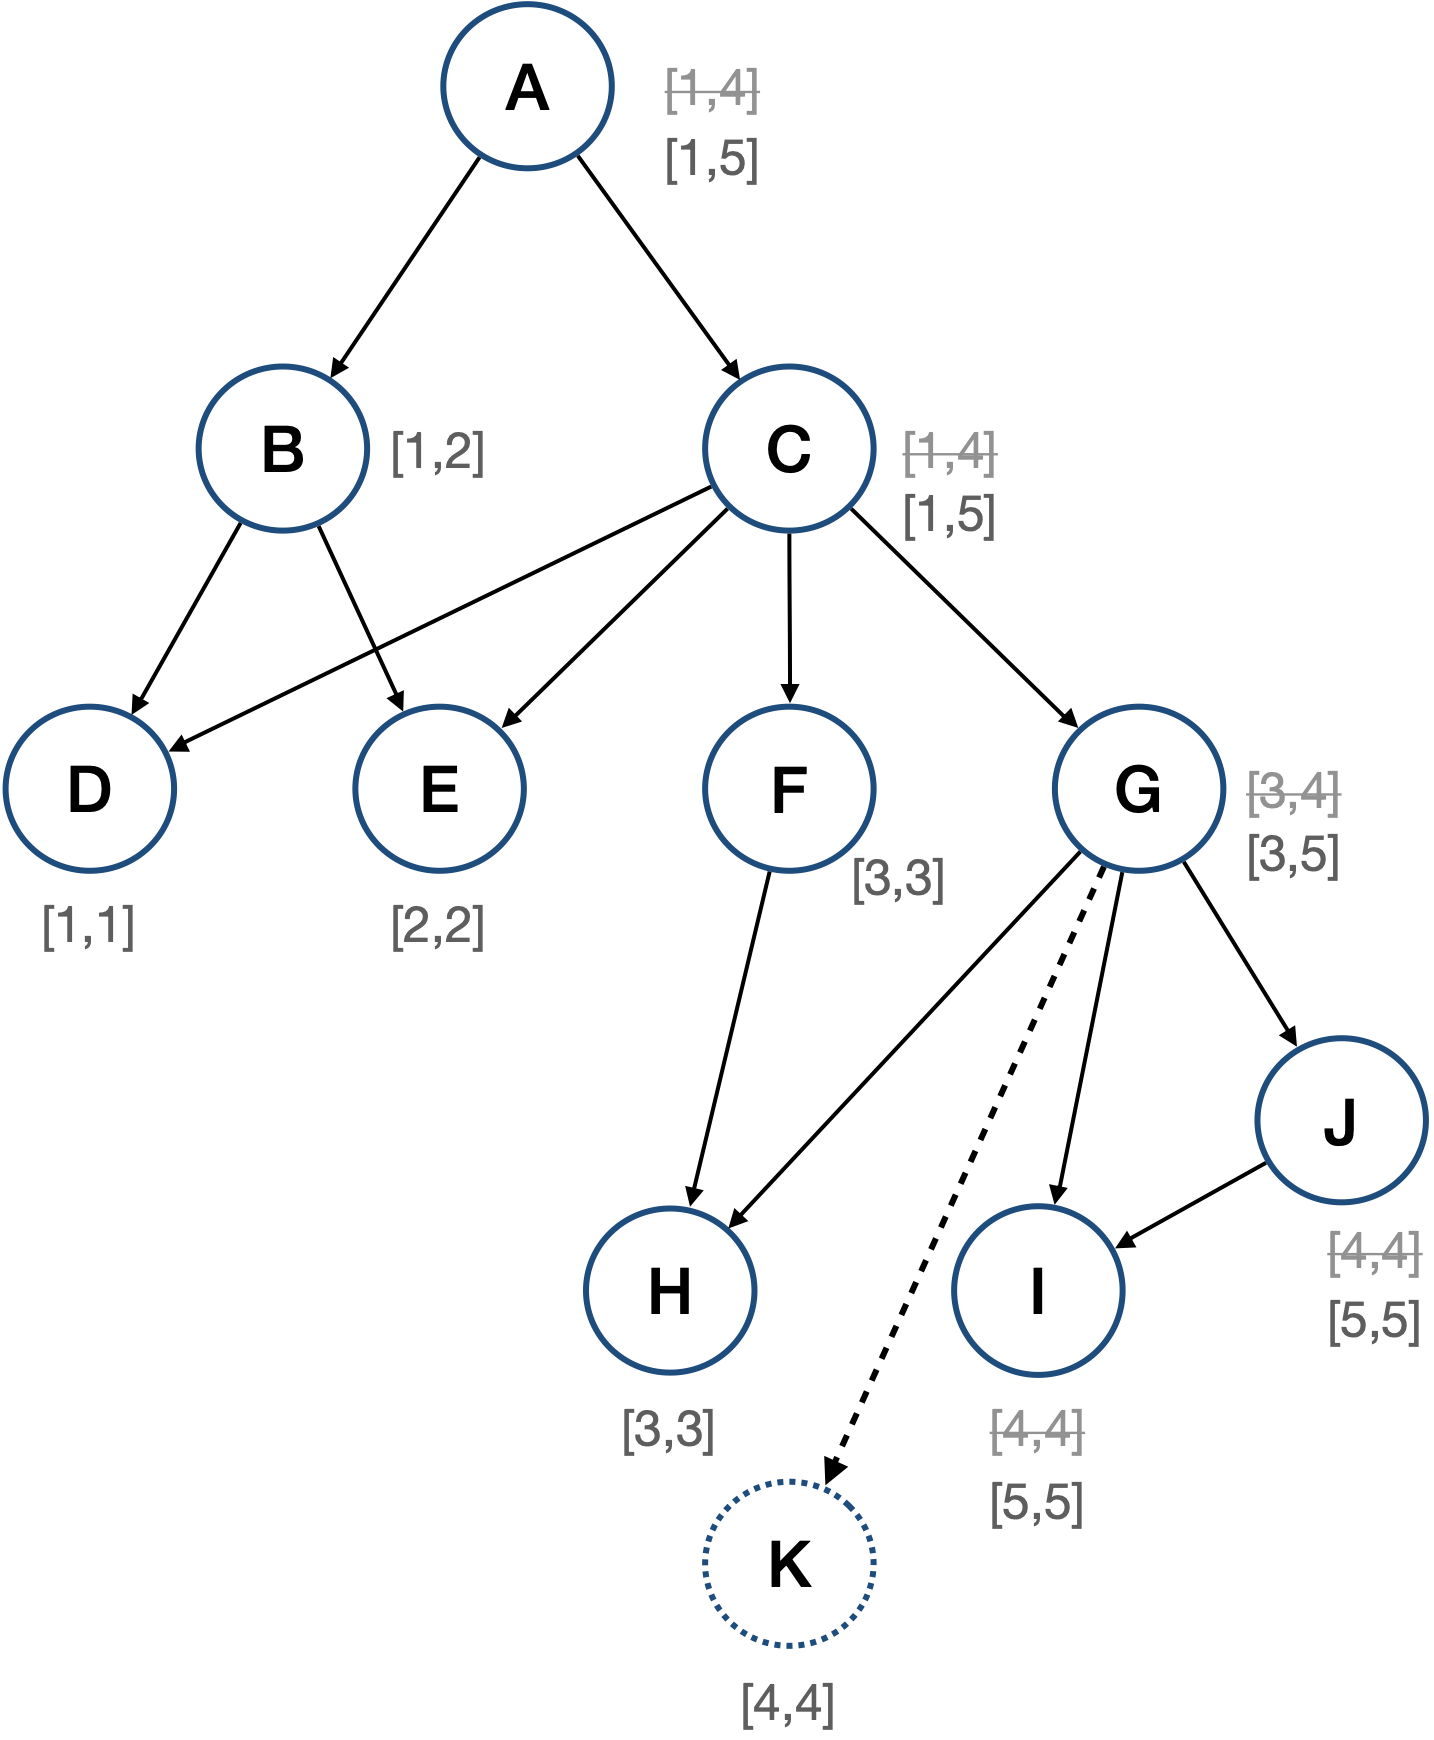
\includegraphics[width=0.6\textwidth]{figures/domlock_example_with_SM.png}
    \caption{DomLock interval recomputation for a vertex insertion}
    \label{fig:domlock_example_SM}
\end{figure}

For example, consider the hierarchy in Figure \ref{fig:domlock_example_SM}. If a vertex $K$ is added as a child of $G$ after $H$, $K$ can only have interval $[4,4]$. This forces $I$ and $J$ to get interval $[5,5]$ and the interval of $G$ must be recomputed to $[3,5]$. This recomputation has to be done for all the ancestors of $G$ as well up to the root of. 

Furthermore, this recomputation might not be parallelizable with any other access. Since the interval of the root is recomputed as well, any other operation, whether read, write or structural modification, has to wait until the recomputation of the root is complete. 
% This is done in order to prevent incorrect dominator identification due to improper intervals.
In order to prevent concurrent accesses from interfering with the recomputation, a structural modification is performed by acquiring a write lock on the root of a hierarchy. This blocks all other accesses until the structural modification and the interval recomputation is complete. 

% In dynamic hierarchies with structural modifications can lead to a significant performance penalty due to the lack of parallelism in the relabelling. 

While DomLock addresses requirement \Rb, false subsumptions and the lack of support for dynamic hierarchies incur significant penalties against requirement \Rc and \Rd respectively.



\subsection{Multi Interval DomLock (MID)}
Multi Interval DomLock \cite{anjuMID} is a successor to DomLock that uses a pair of intervals per vertex to identify the immediate dominator. MID maintains, in addition to a DomLock interval, another interval computed by a reverse post-order traversal of the hierarchy, called the \emph{"DFS-on-image"}. Figure \ref{fig:MID_example_locked} shows the MID intervals for a hierarchy. 

\subsubsection{Preprocessing and Metadata}

A vertex $v$ is labelled with two intervals: the $\mathcal{D}$ interval ($\mathit{ID}_v = [\mathit{lD}_v, \mathit{rD}_v]$) and the $\mathcal{M}$ interval ($\mathit{IM} = [\mathit{lM}_v, \mathit{rM}_v]$). The only difference between the two intervals is the order of traversal used to compute them. $\mathcal{D}$ intervals being post-order and $\mathcal{M}$ intervals being reverse post-order. Leaves of the hierarchy are labelled with unit $\mathcal{D}$ and $\mathcal{M}$ intervals. 
% \begin{figure}[h]
%     \centering
%     \captionsetup{justification=centering}
%     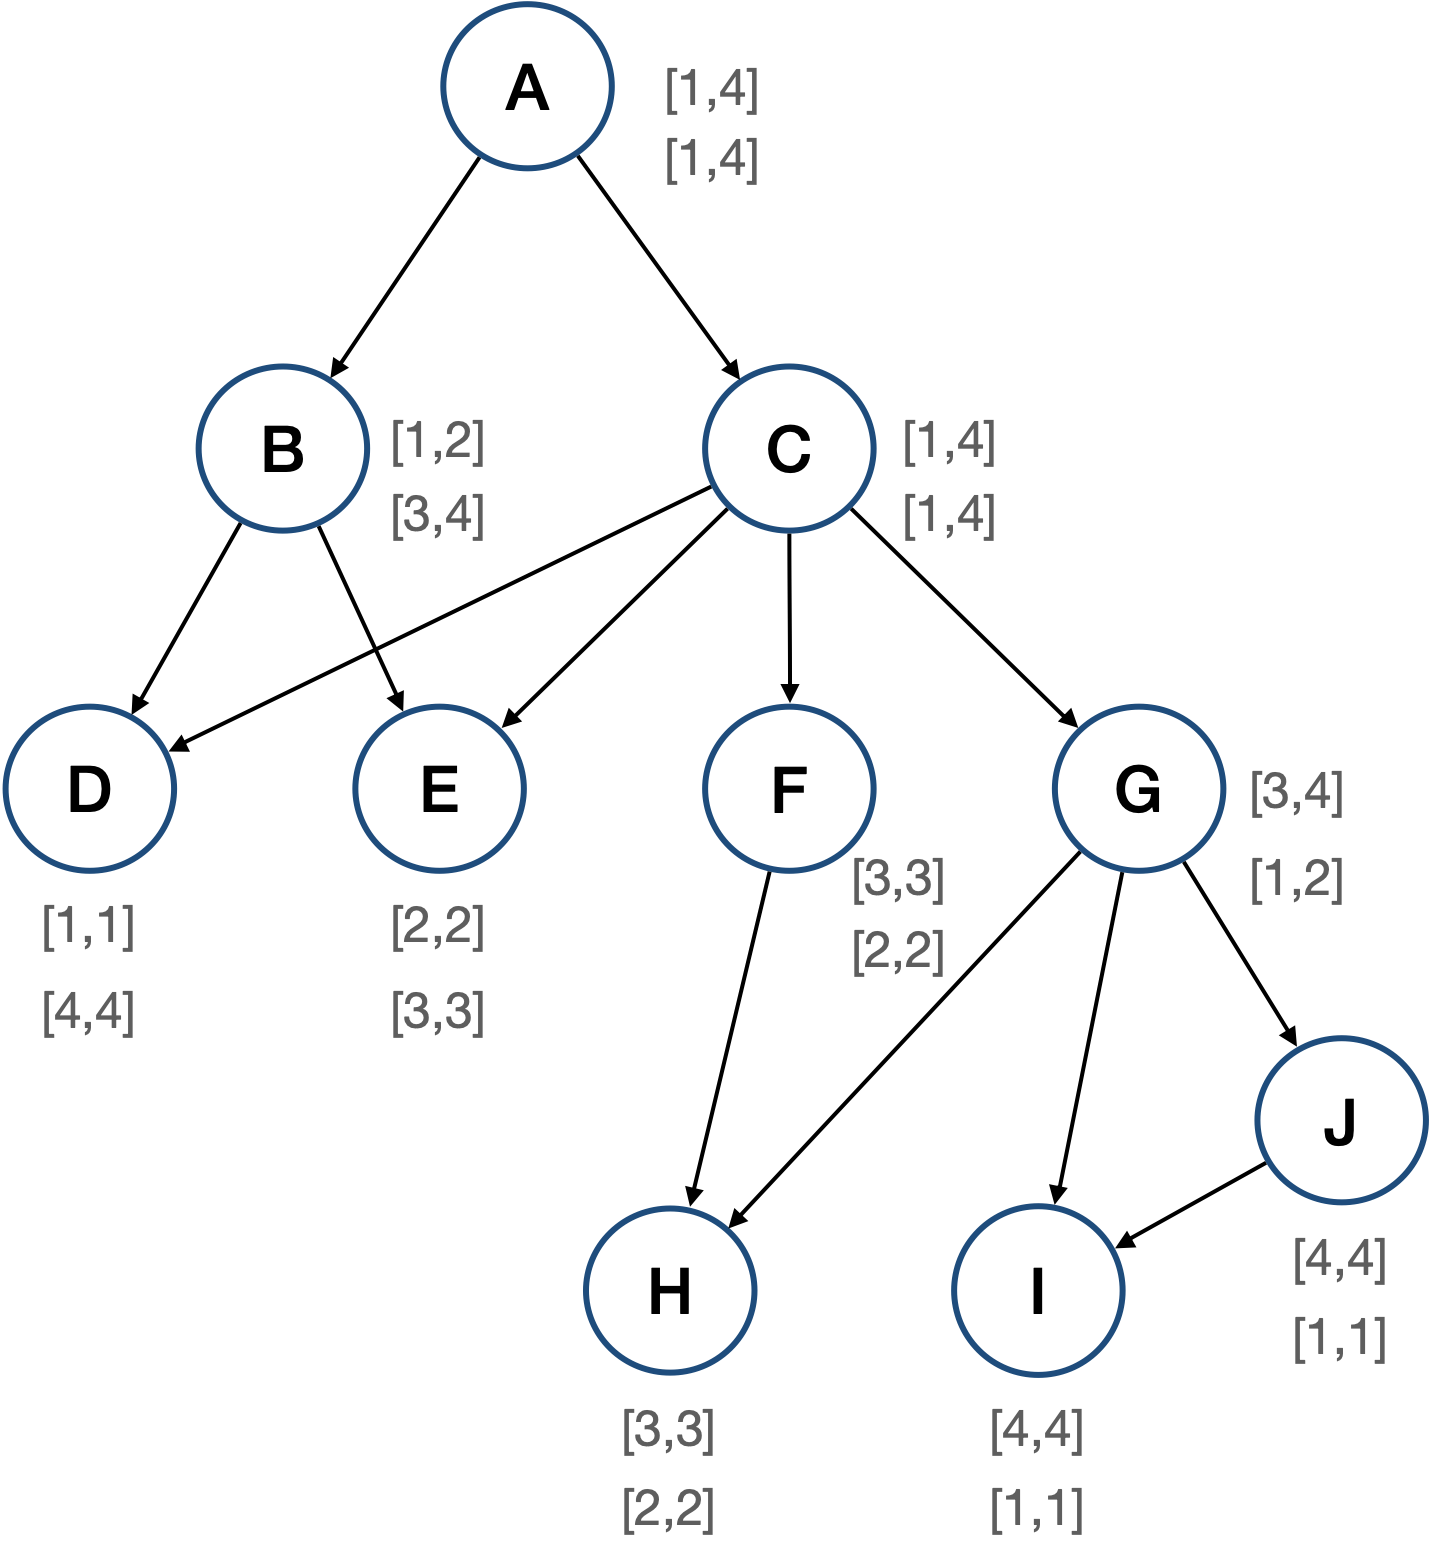
\includegraphics[width=0.5\textwidth]{figures/MID_example.png}
%     \caption{Hierarchy labelled with a pair of intervals: DomLock (top) and MID (bottom)}
%     \label{fig:MID_example}
% \end{figure}

For example, in Figure \ref{fig:MID_example_locked}, vertex $H$ is labelled with $\mathcal{M}$ interval $[2,2]$ in addition to its $\mathcal{D}$ interval $[3,3]$ since it is the second vertex in the reverse post-order traversal. Like DomLock the interval of an internal vertex is computed using the intervals of its children. For both, $\mathcal{D}$ and $\mathcal{M}$ intervals of a vertex, the $l$ value of an internal vertex $v$ is the minimum of the $l$ values of the respective interval of its children and the $r$ value of an internal vertex $v$ is the maximum of the $r$ values of the respective interval of its children.

For example, in Figure \ref{fig:MID_example_locked}, vertex $G$ has three children $H$, $I$ and $J$. The $\mathcal{D}$ and $\mathcal{M}$ intervals of $G$ are $[3,4]$ and $[1,2]$ respectively, since the minimum $l$ values of its children is 3 and 1 and the maximum $r$ values of its children are 4 and 2 respectively.

Intervals of a vertex $u$ subsume ($\prec$) overlapping intervals of all descendants of $u$. A vertex $u$ is a dominator of another vertex $v$ if both, $\mathcal{D}$ and $\mathcal{M}$ intervals of $u$ subsume the respective intervals of $v$.
Subsumption is defined as follows:

\begin{equation}
    \begin{split}
        & u \text{ is a dominator of } v \iff ID_u \prec ID_v \land IM_u \prec IM_v
        \\ & \iff \mathit{lD}_v \leq \mathit{lD}_u \land \mathit{rD}_v \geq \mathit{rD}_u \land \mathit{lM}_v \leq \mathit{lM}_u \land \mathit{rM}_v \geq \mathit{rM}_u
    \end{split}
\end{equation}

For example, in Figure \ref{fig:MID_example_locked}, $G$ is a dominator of $F$, $H$, $I$ and $J$ since both $\mathcal{D}$ and $\mathcal{M}$ intervals of $G$ subsume the respective $\mathcal{D}$ and $\mathcal{M}$ intervals of $F$, $H$, $I$ and $J$.

\subsubsection{Lock Acquisition and Conflicts}
In order to identify the lock grain, MID uses the $\mathcal{D}$ and $\mathcal{M}$ intervals of the targets of a lock request. The immediate dominator is chosen as the lock guard. The immediate dominator, with MID, is the deepest vertex that subsumes the $\mathcal{D}$ and $\mathcal{M}$ intervals of the lock targets. Like DomLock, finding the immediate dominator involves a depth-first search from the root of the hierarchy.

For example, in Figure \ref{fig:MID_example_locked}, suppose a thread wants to acquire a lock on vertices $H$ and $J$ with $\mathcal{D}$ intervals $[3,3]$ and $[4,4]$ and $\mathcal{M}$ intervals $[2,2]$ and $[3,3]$ respectively. The lock guard is a vertex with $\mathcal{D}$ interval $[3,4]$ and $\mathcal{M}$ interval $[1,2]$. A depth first search identifies $G$ as the lock guard for this lock request. 

% The two pairs of intervals are used in an attempt to reduce \emph{false subsumptions} where a vertex subsumes its siblings. When testing subsumption in MID, the two intervals are tested for overlap. A vertex $v$ with intervals $[\mathit{lD}_{v1}, r_{v1}]$ and $[l_{v2}, r_{v2}]$, subsumes another vertex $u$ with intervals $[l_{u1}, r_{u1} ]$ and $[l_{u2}, r_{u2}]$ iff $r_{u1} \land l_{u1} \leq r_{v1} \land l_{v2} \leq r_{u2} \land l_{u2} \leq r_{v2}$.

\begin{figure}[H]
    \centering
    \captionsetup{justification=centering}
    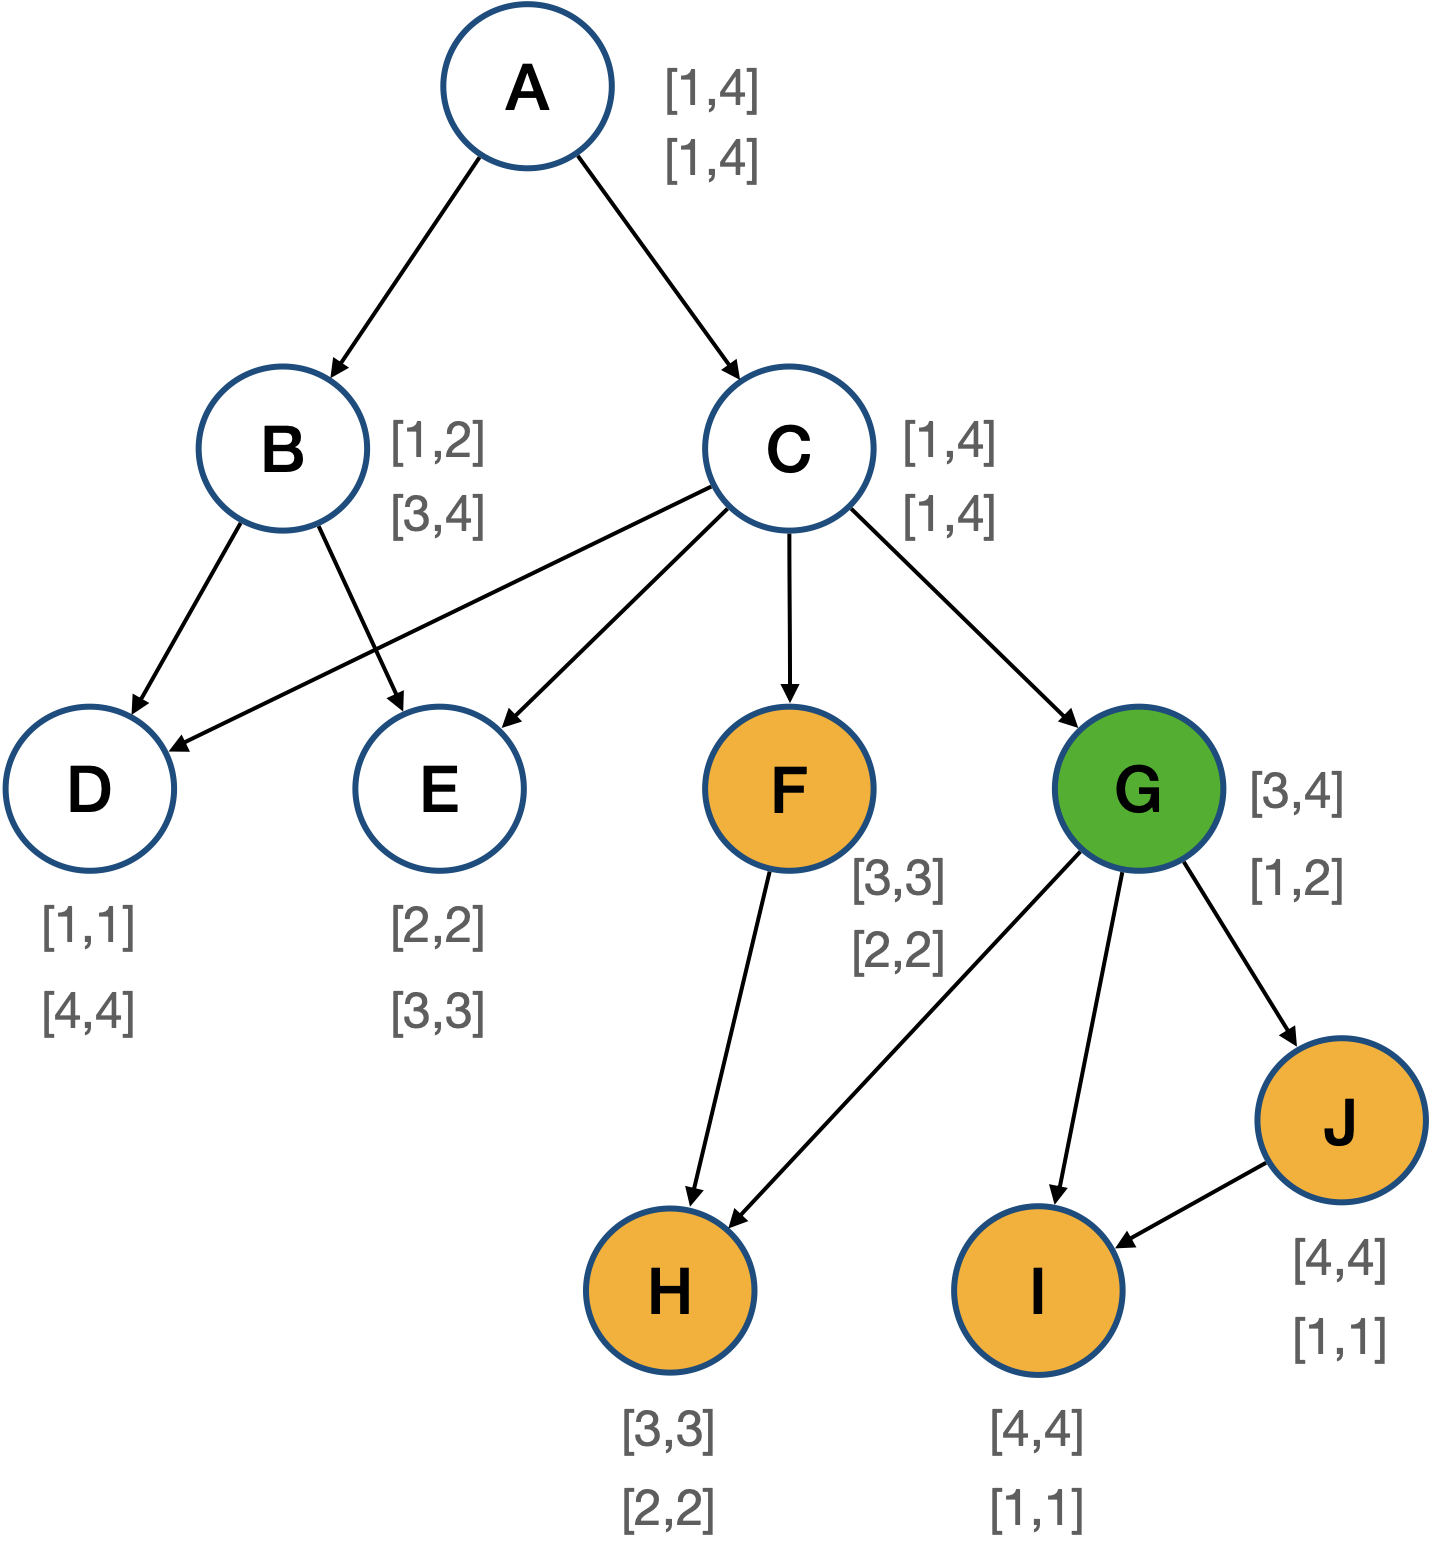
\includegraphics[width=0.6\textwidth]{figures/MID_example_with_lock.png}
    \caption{MID labels with lock on guard $G$ with the grain of the lock (yellow)}
    \label{fig:MID_example_locked}
\end{figure}


The property of subsumption is used to identify the lock grain of a guard in MID. However, unlike DomLock, subsumption is tested on  both $\mathcal{D}$ and $\mathcal{M}$ intervals. 
This is done in an effort to reduce the number of false subsumptions. However, MID still suffers from false subsumptions.


For example in Figure \ref{fig:MID_example_locked}, $G$ subsumes $F$, $H$, $I$ and $J$ since both intervals of $G$ overlap with the respective intervals of $F$, $H$, $I$ and $J$. $G$ subsumes $F$ but $F$ is not a descendant of $G$. A thread that wishes to lock $F$ when $G$ is locked will be blocked due to $F$ and $G$ being included in the same grain even though topologically, they are not. Like DomLock, MID also suffers from poor performance due to such spurious conflicts.

Grain conflicts are identified by testing the $\mathcal{D}$ and $\mathcal{M}$ intervals of the lock guards for overlap. The grains of two lock guards are disjoint only if both $\mathcal{D}$ and $\mathcal{M}$ intervals are disjoint. Two disjoint grains can be locked concurrently. 

\subsubsection{Metadata Maintenance}

MID encounters double the penalty for recomputing vertex labels in dynamic hierarchies when a structural modification occurs. Since two intervals are computed per vertex, both a post-order and a reverse post-order traversal is required to recompute them when a structural modification occurs. In certain cases, the intervals of all vertices are recomputed which is extremely expensive for large hierarchies.

\begin{figure}[H]
    \centering
    \captionsetup{justification=centering}
    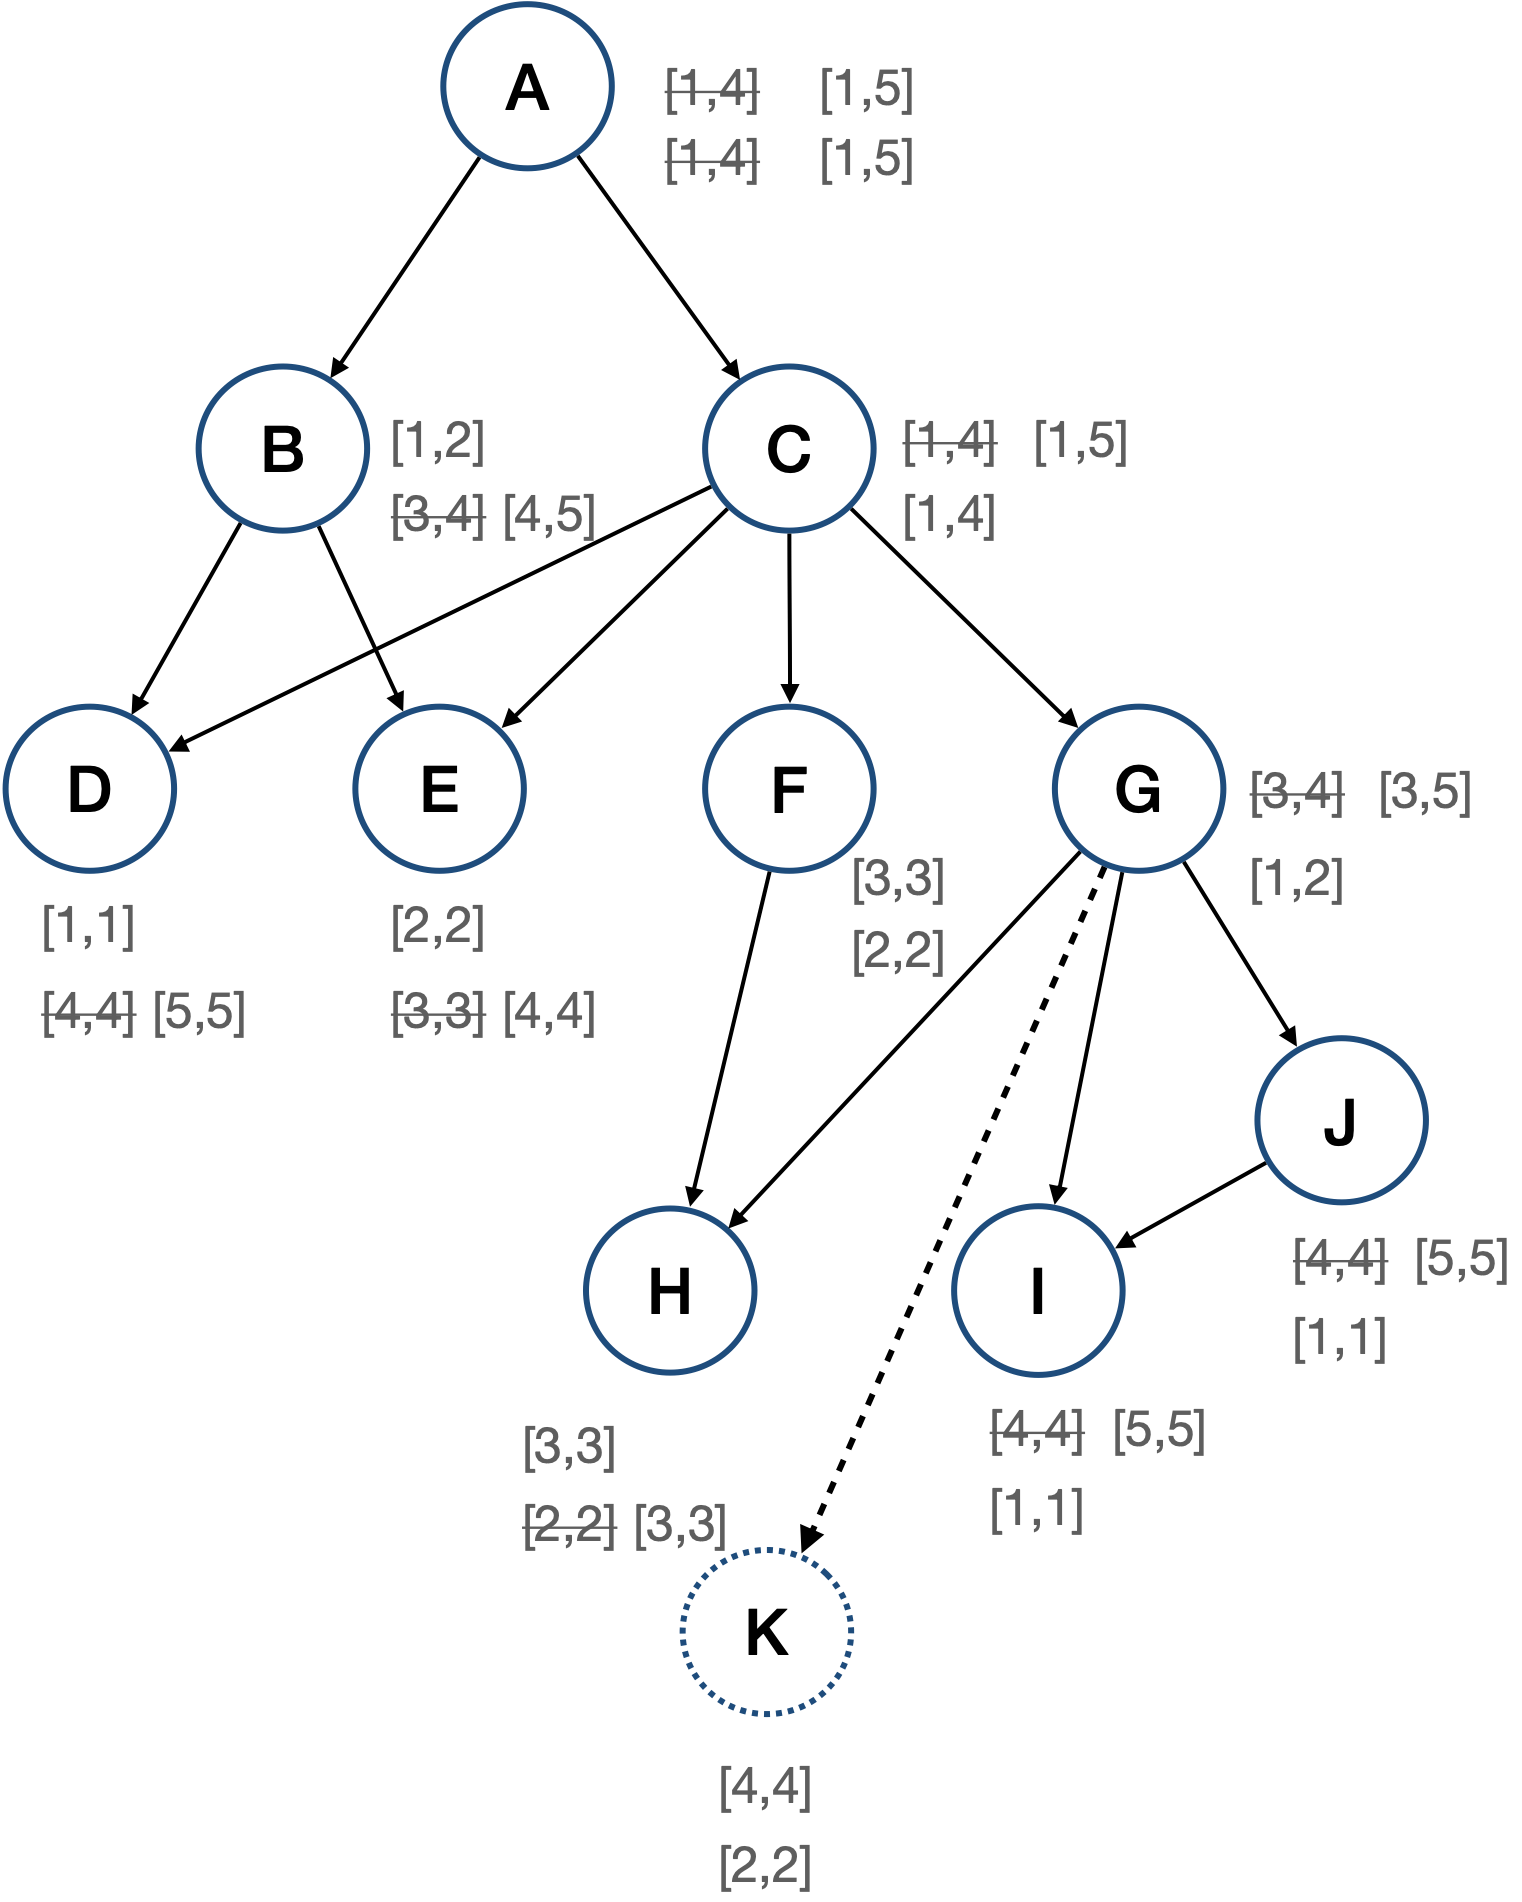
\includegraphics[width=0.6\textwidth]{figures/MID_example_with_SM.png}
    \caption{MID interval recomputation for a vertex insertion}
    \label{fig:MID_example_SM}
    
\end{figure}

For example, when vertex $K$ is inserted as a child of $G$ as shown in Figure \ref{fig:MID_example_SM}, at least one interval for every vertex is recomputed. These intervals are then propagated to the root of the hierarchy. Compared to DomLock, MID relabels more vertices for the same structural modification. 


Like DomLock, to prevent concurrent reads from interfering with the recomputation a structural modification is performed by acquiring a write lock on the root of the hierarchy.

% the hierarchy is guarded by a mutex until the recomputation is complete.

MID tries to reduce false subsumptions w.r.t to DomLock but does not eliminate them completely. The performance penalty for recomputation in dynamic hierarchies is significantly higher in MID as compared to DomLock. As such, MID fulfills requirement \Rb but incurs even severe penalties, compared to DomLock, against requirements \Rc and \Rd.

\subsection{Flexible granularity Locking (FlexiGran)}

FlexiGran \cite{FlexiGran2024} aims to enable both MGL via DomLock, and fine-grain locks to co-exist on the same hierarchy. 
% DomLock is used as the MGL locking technique in FlexiGran and the fixed-grain locks are fine-grain locks i.e. every vertex is its own guard. 
FlexiGran uses the DomLock intervals  as vertex labels and uses vertex depth to determine ancestor-descendent relationships between identical intervals.

\begin{figure}
    \centering
    \captionsetup{justification=centering}
    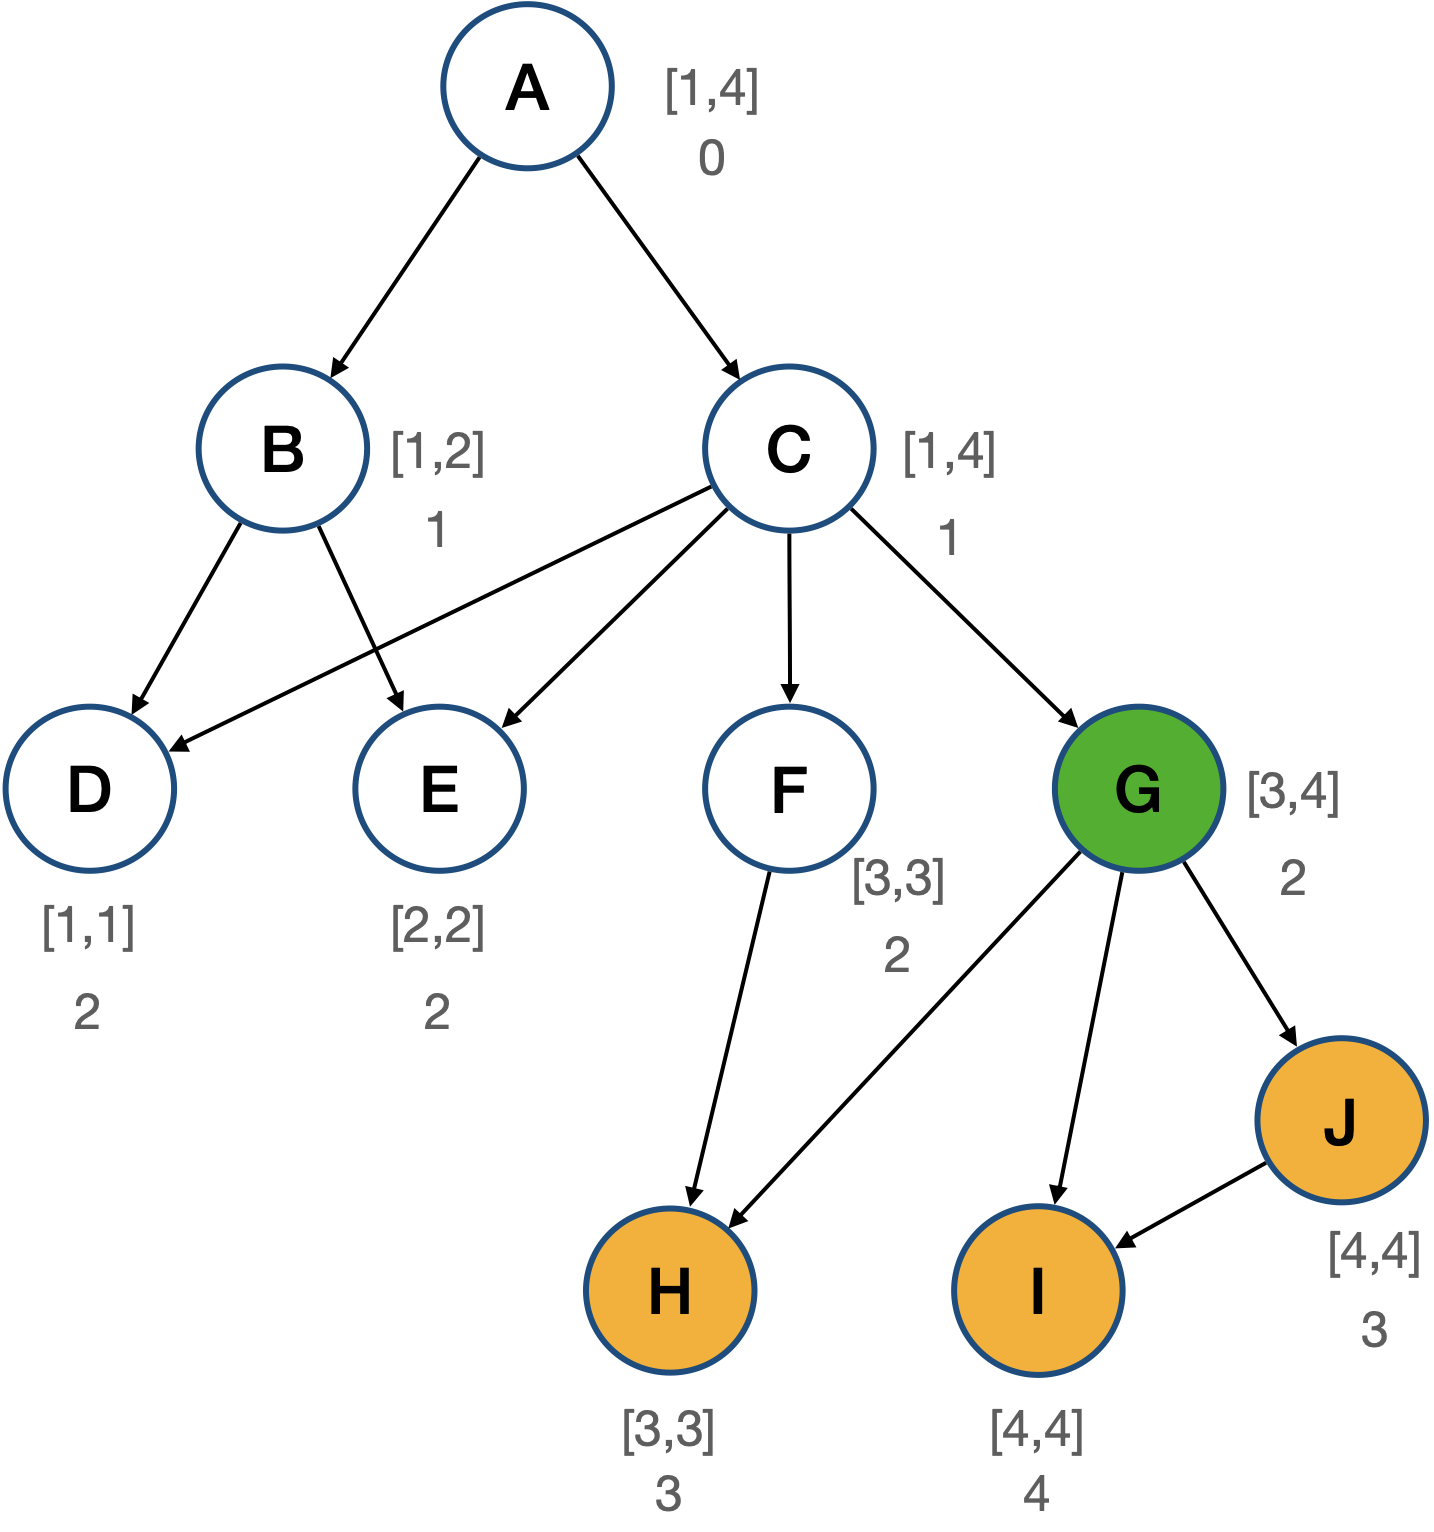
\includegraphics[width=0.5\textwidth]{figures/flexigran_example_with_lock.png}
    \caption{FlexiGran labels and vertex depth with lock on guard $G$ with the grain of the lock (yellow)}
    \label{fig:flexigran_example_locked}
\end{figure}

\subsubsection{Preprocessing and Metadata}

In FlexiGran, a post-order traversal is performed to compute the labels of vertices. Like DomLock, the leaves of the hierarchy are labelled with unit intervals and internal vertices are labelled with intervals computed from the intervals of their children. In addition to these intervals, FlexiGran also computes the depth of each vertex in the hierarchy. The depth of a vertex is the length of the shortest-longest path from the root to the vertex. Figure \ref{fig:flexigran_example_locked} shows the intervals and vertex depths of a hierarchy labelled with FlexiGran.

This shortest-longest path is useful for depth determination in the presence of connected components like cycles. In a cycle, the path is recursive and based on the method of computation, the longest path can be infinite. The shortest-longest path limits this recursion to the length of a path from the root to a vertex which contains the target vertex at most twice, as is the case with cycles. 

\subsubsection{Lock Acquisition and Conflicts}

% FlexiGran uses vertex depth in addition to intervals to determine if two vertices might have an ancestor-descendant relationship between them. 
If a thread requests a MGL lock on a vertex via flexigran, then a lock is acquired via the DomLock protocol by performing a depth first search to find the immediate dominator of the target vertex.
If a thread requests a fine-grain lock, then a read/write lock is directly requested on the target. 

Since both fine-grain and MGL locks can exist in flexigran, the process of testing lock conflicts involves multiple steps. Table \ref{tab:flexigran_locks} shows the compatibility matrix for FlexiGran locks. \textbf{F} and \textbf{H} indicate the kind of lock acquired, fine-grain lock and multi-granularity lock respectively. \textbf{R} and \textbf{W} indicate the lock mode. So, \textbf{FR} is a fine-grain read lock.

When checking if two MGL are compatible, the intervals of their guards are tested for overlap. Disjoint intervals indicate that the two locks are DomLock compatible. When checking two fine-grain locks for conflict, the lock guards for the lock requests are compared. If two fine-grain lock requests are on the same vertex, then they are in conflict if at-least one of the requests is for a write lock.


\begin{table}[h]
    \centering
    \captionsetup{justification=centering}
    \begin{tabular}{c|cccc|cccc|}
        \multicolumn{1}{c}{} & \multicolumn{4}{c|}{\textbf{Lock On Ancestor}} & \multicolumn{4}{c}{\textbf{Lock On Descendent}} \\
        \cline{2-9}
        \textbf{Lock Mode} & \textbf{FR} & \textbf{FW} & \textbf{HR} & \textbf{HW} & \textbf{FR} & \textbf{FW} & \textbf{HR} & \textbf{HW} \\
        \hline
        \textbf{FR} & \cellcolor{green!25} Y & \cellcolor{green!25} Y & \cellcolor{green!25} Y & \cellcolor{red!25} N & \cellcolor{green!25} Y & \cellcolor{green!25} Y & \cellcolor{green!25} Y & \cellcolor{green!25} Y \\
        \textbf{FW} & \cellcolor{green!25} Y & \cellcolor{green!25} Y & \cellcolor{red!25} N & \cellcolor{red!25} N & \cellcolor{green!25} Y & \cellcolor{green!25} Y & \cellcolor{green!25} Y & \cellcolor{green!25} Y \\
        \textbf{HR} & \cellcolor{green!25} Y & \cellcolor{green!25} Y & \cellcolor{green!25} Y & \cellcolor{red!25} N & \cellcolor{green!25} Y & \cellcolor{red!25} N & \cellcolor{green!25} Y & \cellcolor{red!25} N \\
        \textbf{HW} & \cellcolor{green!25} Y & \cellcolor{green!25} Y & \cellcolor{red!25} N & \cellcolor{red!25} N & \cellcolor{red!25} N & \cellcolor{red!25} N & \cellcolor{red!25} N & \cellcolor{red!25} N \\
    \end{tabular}
    \caption{Flexigran compatibility matrix showing the protocol for the co-existence of hierarchical and fine-grained locks in a system. \textbf{F}: Fine-grained, \textbf{H}: Hierarchical, \textbf{R}:Read, \textbf{W}: Write}
    \label{tab:flexigran_locks}
\end{table}

To test the compatibility of a MGL lock with a fine-grain lock, it is necessary to perform reachability check between the guards of the MGL lock and the fine-grain lock. To do so, a search is initiated from the guard of the MGL lock and if the fine-grain lock guard is reachable from the MGL lock guard, then the two locks are incompatible since they lie in the same MGL grain. 

For example, in Figure \ref{fig:flexigran_example_locked}, a hierarchical lock is acquired on $G$. This lock guards vertices $H$, $I$ and $J$. If a fine-grain lock is requested on $F$, it would be compatible with the hierarchical lock on $G$ since there is no path from $G$ to $F$ or vice-versa. Unlike DomLock and MID, A FlexiGran lock on $G$ does not subsume $F$ as $F$ is not a descendant of $G$ since their depths are same.

\subsubsection{Metadata Maintenance}

Like DomLock, structural modifications in FlexiGran require recomputation of the intervals of the vertices. A single post-order traversal is enough to recompute the intervals and depths of vertices. 

Like DomLock a structural modification with FlexiGran is performed by acquiring a write lock on the root of the hierarchy, since the root might be relabelled.

In summary, FlexiGran fulfills requirement \Rb and incurs a significant performance penalty against requirement \Rc due to the expensive compatibility checks required to detect conflicts between MGL and fine-grain locks. FlexiGran also incurs a performance penalty against requirement \Rd due to the non-parallel recomputation of intervals in dynamic hierarchies.



\section{Trade-offs between state-of-the-art techniques}

Recall the primary requirements identified for MGL:
\begin{itemize}
    \item[\Rb] Finding an appropriate lock guard for a lock request.
    \item[\Rc] Efficiently Detecting conflicts between locks
    \item[\Rd] Housekeeping the metadata required to implement the locking protocol.
\end{itemize}

\begin{figure}[h]
    \centering
    \captionsetup{justification=centering}
    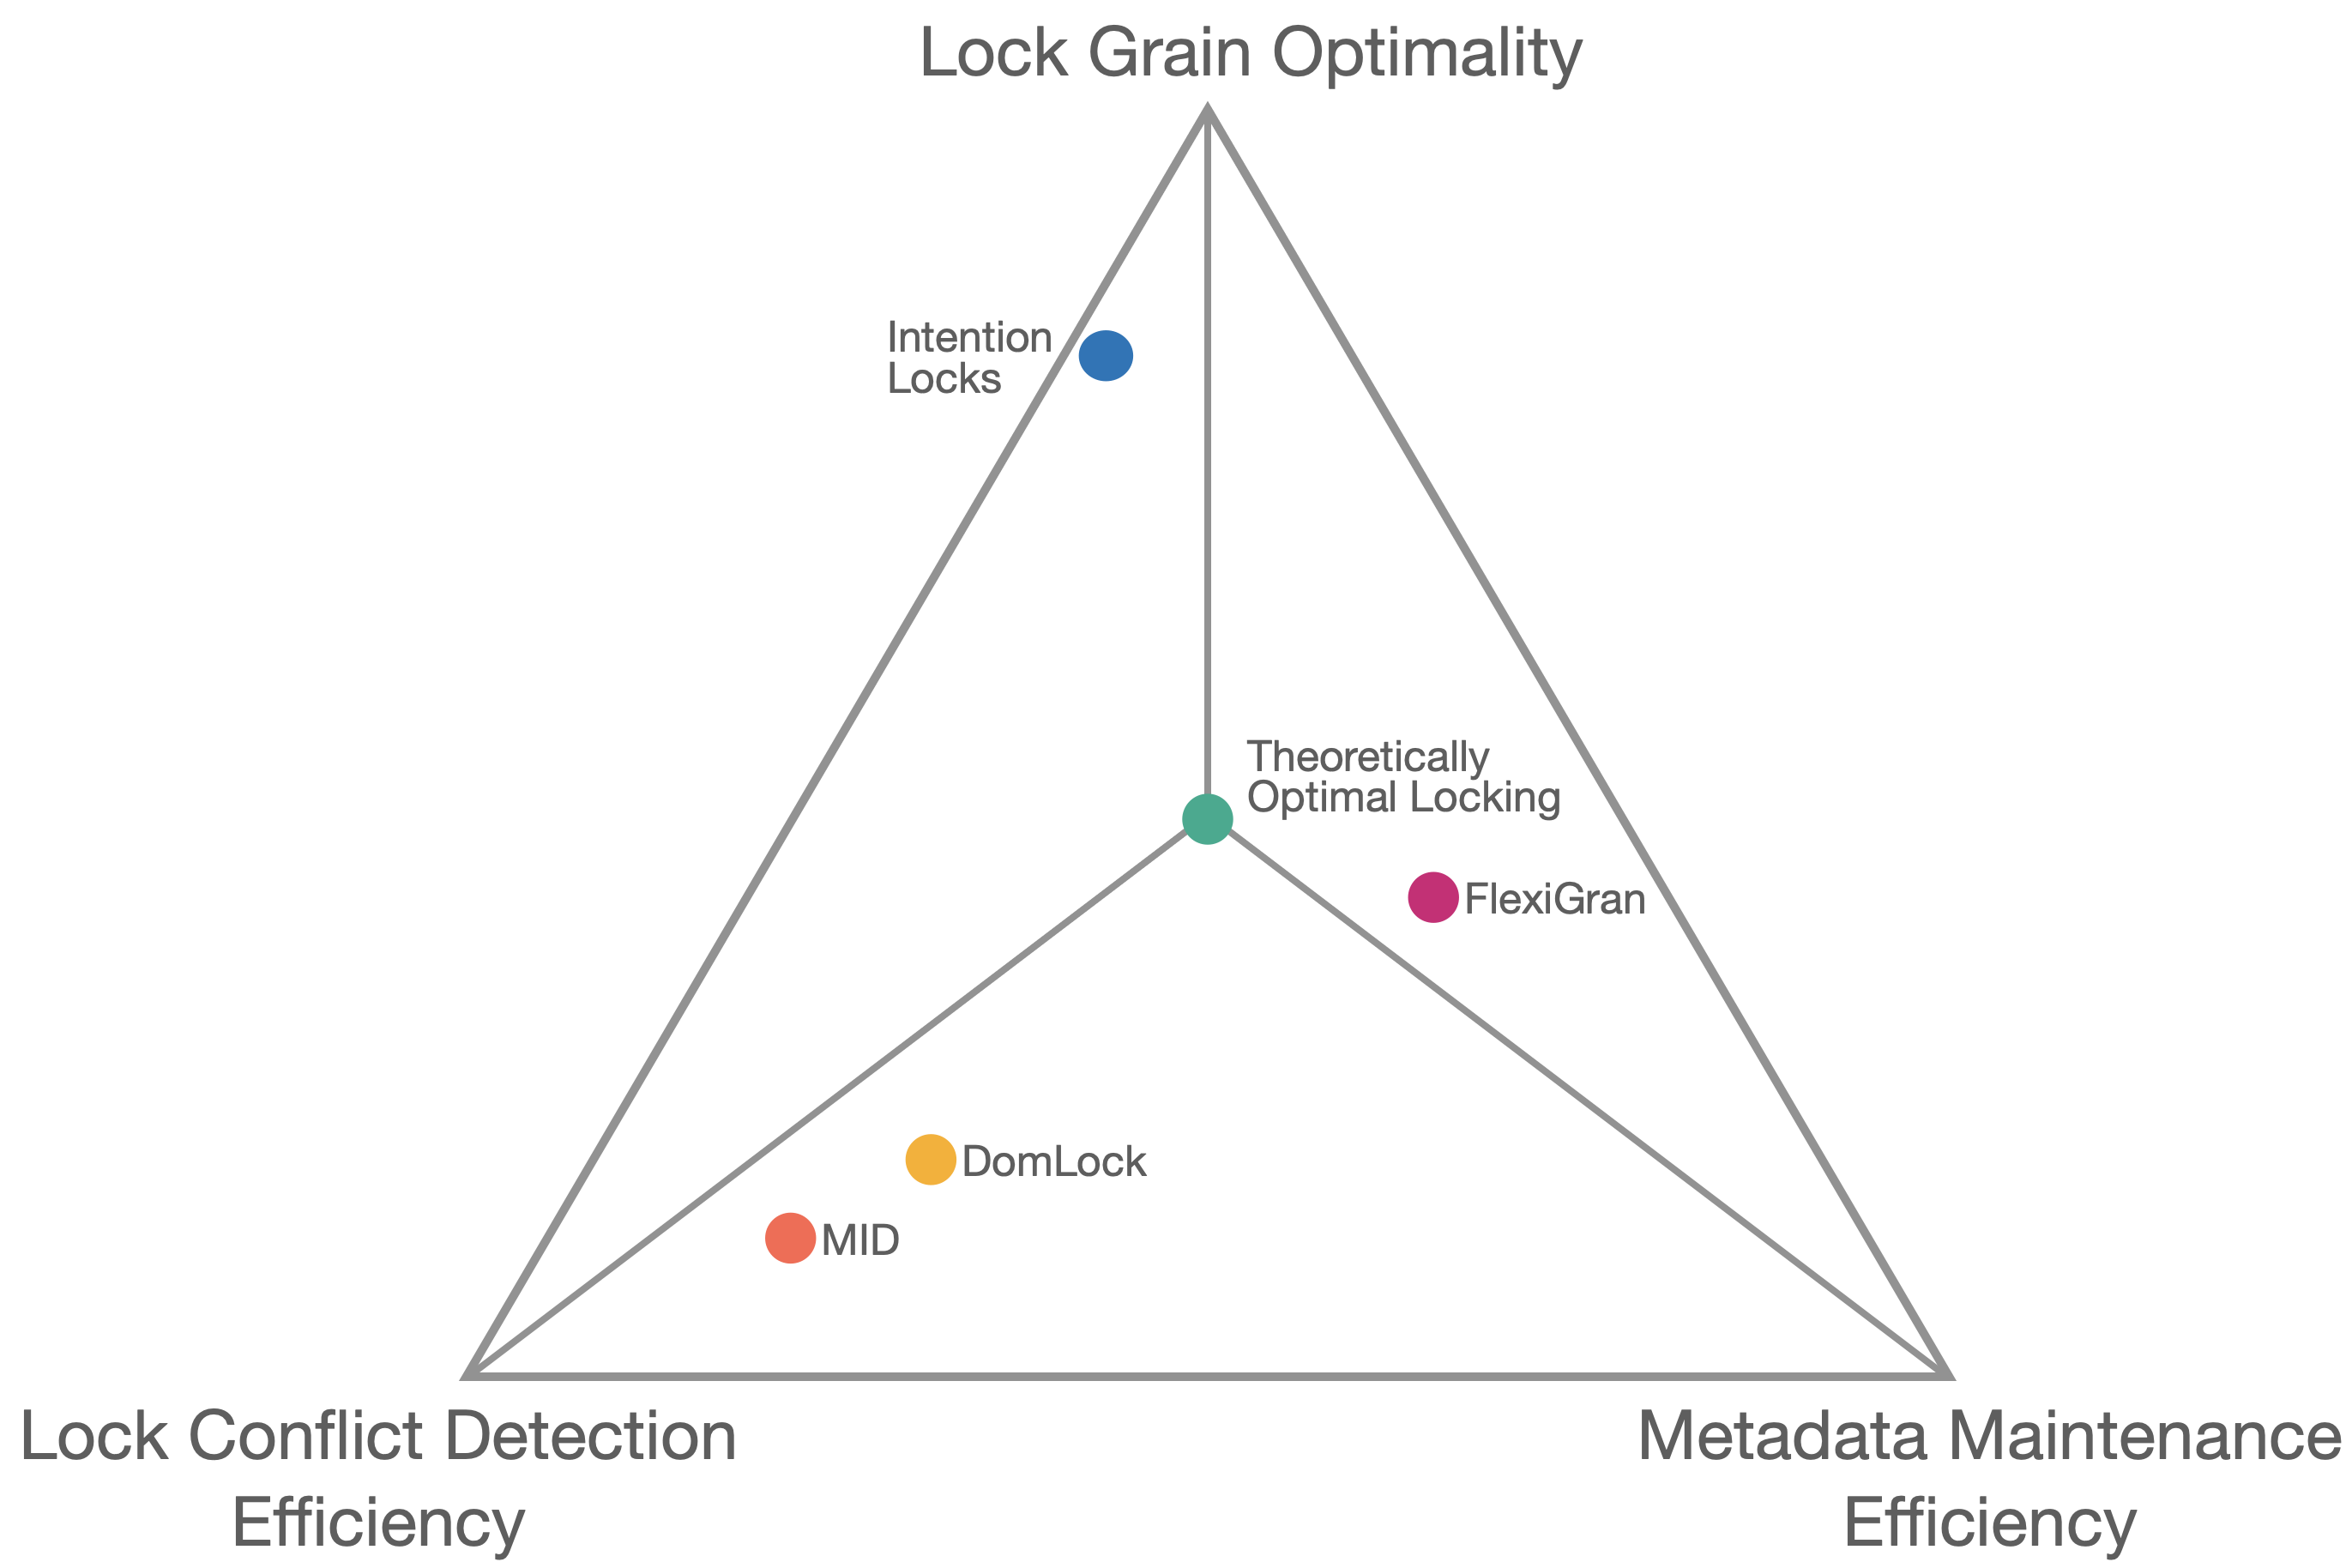
\includegraphics[width=.9\textwidth]{figures/MGL_comparision.png}
    \caption{Trade-offs in MGL techniques}
    \label{fig:tradeoffs}
\end{figure}


MGL based only on paths, like Intention Lock, fulfills requirement \Rb but incurs a significant performance penalty against requirement \Rc due to the number of traversals required to lock a vertex and detect conflicts.

\begin{table}[h]
    \centering
    \captionsetup{justification=centering}
    \begin{tabular}{l | ccc}
        \textbf{Algorithm}  & \Rb & \Rc & \Rd \\
        \hline
        % Coarse-grain Locks & \cellcolor{red!25} N & \cellcolor{green!25} Y &  \cellcolor{gray!25} NA \\
        % Fine-grain Locks & \cellcolor{green!25} Y & \cellcolor{green!25} Y &  \cellcolor{gray!25} NA \\
        % Level-based locks  & \cellcolor{red!25} N & \cellcolor{red!25} N & \cellcolor{red!25} N \\
        Intention Lock & \cellcolor{green!25} Y & \cellcolor{red!25} N & \cellcolor{gray!25} N/A \\
        DomLock & \cellcolor{red!25} N & \cellcolor{green!25} Y & \cellcolor{red!25} N \\
        MID & \cellcolor{red!25} N & \cellcolor{green!25} Y & \cellcolor{red!25} N \\
        FlexiGran & \cellcolor{red!25} N & \cellcolor{green!25} Y & \cellcolor{red!25} N \\
        CALock & \cellcolor{green!25} Y & \cellcolor{green!25} Y & \cellcolor{green!25} Y \\
        
    \end{tabular}
    \caption{Comparison of MGL techniques against requirements}
    \label{tab:tradeoffs}
\end{table}

MGL using labels based on a vertex order such as DomLock, MID and FlexiGran, fulfil requirement \Rb and incur a penalty due to false subsumptions. In addition, due to the metadata required to implement the locking protocol, these techniques incur a performance penalty against requirement \Rd as well when structural modifications occur. 


Figure \ref{fig:tradeoffs} and Table \ref{tab:tradeoffs} shows the trade-offs in the different MGL techniques. Intention locks offer the smallest lock grains at the cost of lock conflict detection. DomLock and MID offer efficient conflict detection at the cost of metadata management. FlexiGran offers better lock grains than others but incurs a performance penalty due to the expensive lock conflict detection. None of the techniques balances all the requirements to come close to an balanced MGL protocol.



\section{Improving efficiency of MGL techniques}

The locking techniques discussed in chapter \ref{chap:relatedwork} are based on the topology of the graph or the nature of the workload. Most MGL techniques enforce an ordering of vertices, either via reachability thereby utilizing paths to vertices, or by a static ordering that ignores the topology of the hierarchy.

\subsection{Path based techniques}
Path based techniques like lock coupling \cite{DBLP:journals/acta/BayerS77}  and intention locks \cite{gray1975granularity} utilize paths from the root of a graph to the lock target. Lock coupling uses a pair of locks that are acquired one after the other on a path to the vertex to prevent concurrent access to the vertex. While intention locking places a set of locks on the path to the vertex to prevent concurrent access. These techniques are efficient for trees and tree-like structures where the path to a vertex from the root is unique. However, generalizing these techniques to graphs or even hierarchies is not appropriate. As we will see in Chapter \ref{chap:evaluation}, the performance of Intention locks degrades significantly when locking over hierarchies.

\subsection{Label based techniques}
Other MGL techniques make use of labelling strategies that identify an ordering of vertices which is later used by the locking protocol to identify lock grains. Techniques such as DomLock, MID and FlexiGran fall into this category. By using a predefined ordering, for example a post-order, these techniques can very efficiently identify the lock guard and grain. However, the topological detail of the graph is lost.  

% Other techniques like Toggle \cite{kalikar_toggle_2019} circumvent locking all together and use thread schedulers based on  to prevent race conditions. While scheduling techniques are efficient, they involve redesigning an application and are not readily useable for general developers. 

\subsection{Unified Path and Label based techniques}
Unified techniques for labelling are explored in literature in the domain of metadata management for large scale, efficient searching applications. The Dewey Decimal System \cite{DBLP:journals/jd/Sweeney83} is the earliest example of a path based labelling technique used to identify elements of a hierarchy based on their subclassification. Other path based techniques use similar representations of paths. 

A path based labelling technique that preserves the topological ordering of vertices in the labels and facilitates efficient locking would be an ideal solution. However, the additional metadata required to implement this unified technique should not be prohibitively expensive. DomLock and its successors sacrifice labelling performance for locking performance to an extent that makes them unusable for hierarchies that undergo structural modifications. CALock labelling scheme balances maintaining both topological information of the hierarchy while being efficient for locking and also being efficient for relabelling. 

\section{CALock: A topological multi-granularity locking technique}

We propose a new labeling scheme based on path properties, that supports multi-granularity locking. {\em Common-Ancestor lock} ({\em CALock}) is based on a labeling that efficiently computes the closest common ancestor of a set of vertices in a rooted directed graph.
By choosing the closest guarding common ancestor of a set of lock targets as their guard, CALock minimizes grain size. In using paths, by avoiding a fixed ordering of vertices, CALock circumvents expensive relabelling while providing the same locking guarantees as other MGL techniques. The label of a vertex in the graph is a set of its guarding ancestors, computed recursively via breadth-first traversal which we discuss in chapter \ref{chap:calock}.